\documentclass[11pt, a4paper]{article}

% ---------- Packages ----------
\usepackage[utf8]{inputenc}
\usepackage[T1]{fontenc}
\usepackage{lmodern}
\usepackage[english]{babel}
\usepackage{geometry}
\geometry{margin=2.5cm}

\usepackage{graphicx}          % figures
\usepackage{amsmath, amssymb}  % math
\usepackage{booktabs}          % nice tables
\usepackage{array}
\usepackage{tabularx}
\newcolumntype{Y}{>{\raggedright\arraybackslash}X}
\usepackage[expansion=false,nopatch=footnote]{microtype}
\usepackage{longtable}
\usepackage{pdflscape}
% \usepackage{siunitx}           % aligned numbers / units in tables
\usepackage{caption}
\usepackage{subcaption}        % subfigures
\usepackage{float}             % [H] placement
\usepackage{natbib}            % \citep{}, \citet{}
\usepackage{tikz}              % vector diagrams
\usetikzlibrary{positioning, arrows.meta, shapes.geometric}
\usepackage{hyperref}          % clickable references
\usepackage{cleveref}          % \Cref{}, \cref{} — load AFTER hyperref
\usepackage{authblk}           % author/affiliation blocks
\usepackage{setspace}
\onehalfspacing

% authblk has no built-in \corrauthor command; define a minimal one that
% stores the corresponding author's name/e-mail and prints a footnote
% marker next to their \author entry.
\newcommand{\corrauthor}[3]{%
  \affil[#1]{}% no-op placeholder to keep affil numbering intact if needed
  \gdef\corrauthorname{#2}%
  \gdef\corrauthoremail{#3}%
}
\newcommand{\printcorrauthornote}{%
  \begingroup\footnotesize\noindent
  \textsuperscript{*}Corresponding author: \corrauthorname\ (\href{mailto:\corrauthoremail}{\corrauthoremail})
  \endgroup\par\medskip
}

\hypersetup{
    colorlinks=true,
    linkcolor=blue,
    citecolor=blue,
    urlcolor=blue
}

% ---------- Title ----------
\title{Gap2Idea: A Selective Verification Funnel for Limitations and Future Work}
% \author[1]{}
\author[1]{Yazan~Alnakri}
\author[2]{Osama~Orabi}
\author[3]{Hamza~aldaghstany}
\author[4]{Firas~Jolha}
% \author[5,6]{Giancarlo~Succi}


\affil[1]{Innopolis University, Innopolis, Russia (e-mail: y.alnakri@innopolis.university)}
\affil[2]{Innopolis University, Innopolis, Russia (e-mail: o.orabi@innopolis.university)}
\affil[3]{Innopolis University, Innopolis, Russia (e-mail: h.aldaghstany@innopolis.university)}
\affil[4]{Innopolis University, Innopolis, Russia (e-mail: f.jolha@innopolis.university)}



% \corrauthor[1]{Firas Jolha}{f.jolha@innopolis.university}

\date{4 November 2026}

\begin{document}

\maketitle
% \printcorrauthornote

\begin{abstract}
Scientific papers contain limitations and future-work statements that can support literature
review and research planning, but extracting these statements requires both source attribution
and control of processing cost. We study a three-stage funnel: structural localization,
sentence detection, and selective large-language-model (LLM) verification. The implementation
retains source sentences rather than generating gap descriptions. We evaluate saved experiments
separately for full-article limitation detection, future-work recognition, and an auxiliary
literature-gap task. On a 40-article randomized-trial evaluation stream containing 7,968 sentences
and 205 labelled limitations, localization retains 203 positives while discarding 76.3\% of
sentences. A fine-tuned PubMedBERT detector then achieves precision 0.460, recall 0.878, and
$F_1$ 0.604. Selective verification increases precision to 0.580 and $F_1$ to 0.658, while
reducing recall to 0.761. An estimated input-token comparison on these articles gives
282,846 tokens for full-article prompting versus 75,622 for selective verification, a
3.74-fold reduction; this estimate excludes detector computation and output tokens.
Classical baselines, localization ablations, detector-development studies, and prevalence
sensitivity analyses show that rankings depend on the input condition and target definition.
We also document model-labelled reference construction and a human-validation protocol,
without treating pending annotation as completed evaluation. Because prompts were refined using benchmark feedback, the LLM results
are exploratory rather than untouched-test estimates. The study establishes a measured
precision--recall and input-volume trade-off, without claiming general superiority over
published systems or validation of downstream idea generation.
\end{abstract}

\tableofcontents
\newpage

% ---------- Sections ----------
\section{Introduction}
\label{sec:introduction}

Research papers often tell their readers where a study falls short and what should be investigated
next. In clinical research, self-acknowledged limitations help readers interpret findings in light
of study design, data, and applicability~\citep{kilicoglu2018automatic}. In other disciplines,
future-work statements identify extensions, unresolved questions, and further evaluations that
authors consider worth pursuing~\citep{zhu2019recognizing,zhang2023fws}. We refer to these passages
as \emph{author-stated research gaps}: limitations and future-work directions expressed about the
authors' own work. Their extraction provides a way to make this information searchable without
requiring a model to invent a criticism or a research direction.

A collection of such statements can support several activities. A researcher may look for
recurring restrictions in evaluation, identify settings that authors have left untested, or
compare how studies describe future directions. A reviewer may use extracted statements to
locate the authors' discussion of evidence and applicability. Corpus-level work already analyzes
limitation reporting and future-work categories, and traces whether later publications engage
with earlier research directions~\citep{lan2024automatic,hao2020acl,suray2024future}. These uses
motivate a reliable extraction layer, but their interpretation remains conditional: an author's
statement records a reported limitation or direction, not an independently established open
problem. Later work may have addressed it, and the author may not have acknowledged every
important weakness.

The first challenge is therefore definitional. A sentence criticizing prior research can be
useful in a literature review yet lie outside the extraction of a study's own limitations.
Similarly, a statement about how the current paper extends earlier work need not describe
future research. Annotation schemes distinguish these functions in different ways. Argumentative
zoning and scientific-concept annotation include categories related to gaps, failures, and future
work~\citep{liakata2010corpora}, while full-text resources annotate limitations and rhetorical
roles in separate layers~\citep{fisas2016multilayered}. Sci-Sentence provides explicit
Research Gap, Limitation, and Extension categories for literature-review analysis~\citep{bolanos2025scisentence}.
Their names are related to our objective, but their definitions and attribution targets are not
interchangeable. An extraction study must state which source claims count before comparing methods.

The second challenge is structural. Authors may place limitations in a dedicated section,
within a discussion or conclusion, or alongside a particular methodological choice. Dedicated
sections facilitate localization, but their surrounding text also contains results, mitigation,
contribution claims, and descriptions of other studies. Restricting attention to terminal
sections can remove irrelevant material cheaply, while also excluding mid-paper statements.
PDF reading order, broken hyphenation, and sentence boundaries add a further source of error.
A correct sentence classifier cannot recover a gold statement that the parser or localizer has
already omitted. Evaluating localization and detection separately is therefore necessary to
understand the recall of the complete system.

Prior extraction work provides useful precedents. Clinical limitation recognition uses headings,
lexical cues, and supervised or semi-supervised classifiers~\citep{kilicoglu2018automatic}.
Later work on randomized controlled trials (RCTs) separates limitation-sentence detection from
classification into limitation types~\citep{lan2024automatic}. Future-research recognition in
JASIST articles and future-work recognition in NLP similarly separate locating relevant sentences
from grouping or classifying their content~\citep{zhu2019recognizing,zhang2023fws}.
These studies motivate the use of inexpensive structural and lexical evidence before more
flexible semantic classification. They do not imply that one detector transfers equally well
between biomedical full articles, NLP conclusions, and literature-review sentences.

Large language models (LLMs) offer another route, but they introduce a distinct allocation problem.
A full-article prompt presents many sentences unrelated to the extraction target, whereas a
candidate-only prompt depends on the recall of the earlier stages. LLM-based work also combines
source extraction with generation: LimGen uses author-written limitation sections as reference
material, BAGELS evaluates limitation extraction and generation, and FutureGen extracts and
then generates future-work text~\citep{faizullah2024limgen,alazher2025bagels,alazher2025futuregen}.
Critical-limitation and unstated-limitation studies instead ask models to identify weaknesses
that may not have been explicitly acknowledged~\citep{xu2025llms,mishra2026tree}.
The ability to produce a plausible criticism does not establish the ability to identify an
existing author-stated sentence. Our objective is the latter, with source attribution retained.

We investigate a \emph{selective verification funnel} that divides this extraction task into
three stages. Stage~A selects candidate regions using document structure. Stage~B combines sentence
detection, with lexical cues in the hybrid configuration. Stage~C optionally asks an LLM to verify the surviving candidates
against the task's attribution policy. Each stage selects existing parsed sentences rather than
rewriting them. This design makes the consequences of compression visible: we can measure how
many labelled positives remain after localization, how many candidates the detector passes on,
and which true and false positives the verifier removes.

The present experiments examine this mechanism under several distinct input conditions. The
principal analysis uses reconstructed full-article SAL records from biomedical RCT reports, with
complete saved detector predictions and verifier decisions. Separate studies concern curated
future-work sentences in NLP, a literature-gap classification task, and a small arXiv development
reference. Development studies further compare localizer variants, lexical baselines, class
balancing, and alternative reference sets. A documented model-labelled corpus and its implemented
human-validation workflow are distinguished from completed human evaluation. We also compare estimated LLM input and a recorded small full-article prompting baseline.
Dataset-specific labels, prevalence, and processing units are kept explicit because pooling them
would obscure what each experiment measures. These experiments concern extraction and its
processing requirements; corpus-level characterization is a separate empirical objective.

\paragraph{Research questions.}
We ask three questions for the evidence reported in this paper:
\begin{itemize}
  \item \textbf{RQ1 (Stage contribution).} How do structural localization, sentence detection,
        and selective LLM verification change limitation-detection precision, recall, and $F_1$
        on a full-article stream?
  \item \textbf{RQ2 (Detector and reference dependence).} How does the observed trade-off vary
        across detector families, annotation targets, and reference construction, including
        author-stated future work and literature-gap recognition?
  \item \textbf{RQ3 (Input efficiency).} How much LLM input is avoided by selecting candidate
        sentences, and what effectiveness is recorded in a same-model full-article comparison?
\end{itemize}

\paragraph{Contributions.}
The study makes three contributions:
\begin{enumerate}
  \item An extractive pipeline with explicit interfaces for localization, detection, and
        verification, together with the rationale for allocating structural, lexical, learned,
        and LLM processing to different stages.
  \item A full-article stage analysis recomputed from saved sentence-level predictions and
        verifier decisions, accompanied by detector comparisons and separate auxiliary-task
        results that make the input condition and attribution target visible, alongside development
        ablations and reference-sensitivity analysis.
  \item An input-token accounting study and a small same-model full-article comparison,
        reporting effectiveness and processing-volume trade-offs separately from unmeasured
        total billing or throughput.
\end{enumerate}
Prompt development used benchmark feedback, so the verifier results are exploratory.
The claim is a measured trade-off for the examined configurations, rather than general superiority
of LLMs, independent validation across all disciplines, or demonstrated idea-generation quality.

\paragraph{Paper structure.}
\Cref{S:related-works} develops the literature comparison, including the chronological
study-by-study table. \Cref{S:methodology} traces data acquisition, preparation, extraction,
scoring, and the analyses used to answer each RQ. \Cref{S:results} reports the verified and
aggregate results with their evidence status. \Cref{S:discussion} interprets the mechanisms and
validity limits, and \Cref{S:conclusion} summarizes the answers and the next evaluation steps.

\section{Related Work}
\label{S:related-works}

Our study connects the recognition of author-stated limitations and future work with rhetorical
sentence classification, LLM-supported scholarly-text processing, and analysis of reported research
directions. These areas share input documents and some methods, but their output claims differ.
We review that relationship before positioning the current extraction evaluation.

\subsection{Rhetorical annotation and scientific sentence classification}
\label{S:rw-background}

Argumentative zoning provides an early account of sentences according to their role in scientific
argument~\citep{teufel2002summarizing}. \citet{liakata2010corpora} describe AZ-II alongside Core
Scientific Concepts (CoreSC), illustrating two complementary views of scholarly content. Roles
such as future work, weaknesses in prior research, and failures of an author's approach can all
help locate research-relevant statements, but they do not constitute a single uniform author-gap
label. The attribution target and the distinction between a statement's rhetorical role and its
semantic content remain part of the annotation definition.

Full-text annotation is also an established setting. The Dr.~Inventor corpus contains 40 Computer
Graphics articles with multiple annotation layers, including argumentative roles and statements
about advantages or disadvantages~\citep{fisas2016multilayered}. The presence of limitation and
future-work information in separate layers is relevant to our task: it shows why a joint extraction
interface can draw on earlier annotation work without claiming to introduce the first full-text
resource containing both kinds of statement.

Abstract classification resources offer a different input condition. PubMed~200k~RCT
provides biomedical abstract roles, while CSAbstruct supports classification of computer-science
abstract sentences~\citep{dernoncourt2017pubmed,cohan2019pretrained}.
MAZEA and Emerald~110k broaden the available rhetorical annotation
schemes~\citep{dayrell2012rhetorical,stead2019emerald}. Such resources support document understanding,
but an abstract role such as conclusion or objective does not establish that a sentence expresses
an author-stated limitation. Treating every non-gap-specific role as a reliable negative would
also require checking whether gap statements can occur inside that role.

Context matters for classification because a short sentence may inherit its subject or purpose
from nearby text. \citet{jin2018hierarchical} use a hierarchical sequence model to incorporate
surrounding sentences in medical abstracts. \citet{brack2024sequential} examine cross-domain
multi-task learning for scientific sentence classification, and \citet{lan2024multilabel} study
multi-label classification with LLMs. These studies motivate explicit treatment of context, but
they do not establish that complete-sequence modeling is always appropriate for sparse gap labels
in full papers. \citet{zhang2024extracting} instead investigate context-enhanced problem/method
sentence extraction, an adjacent task in which local context helps interpret a target sentence.
Our verifier uses neighboring source sentences for attribution without replacing the task by
whole-document rhetorical classification.

\subsection{Author-stated limitation recognition}
\label{S:rw-authorstated}

\citet{kilicoglu2018automatic} recognize self-acknowledged limitations in clinical research using
rules and learned approaches. Their heading and lexical evidence provides a direct precedent for
our localization and cue stages. The important relationship is mechanistic: document structure
reduces the search space, while sentence-level evidence distinguishes limitation claims from
surrounding exposition. This is more specific than treating all methods that process scientific
text as equivalent extraction baselines.

\citet{lan2024automatic} extend clinical limitation work to 200 annotated RCT publications with
15 categories and 24 subcategories. Their reported binary detector $F_1$ of 0.821 differs from the
limitation-type classification result. Their at-scale application also characterizes limitation
reporting. The dataset is useful to us because it supplies author-gap labels and non-positive
sentences in an article-based setting. However, a reported candidate-pool recognition score cannot
be compared directly with a reconstructed full-stream score: section filtering, label prevalence,
training choices, and the recall denominator must first be aligned.

LimGen contributes author-written limitation sections from 4,068 ACL papers for suggestive
limitation generation~\citep{faizullah2024limgen}. These sections provide useful reference and
training material, but section membership is a form of supervision rather than proof that every
sentence is a semantic limitation. The distinction matters when a precision filter rejects a
method description, result statement, or checklist item occurring inside a Limitations section.
Nor is the original generation task an official binary-detection baseline simply because its
references can be transformed into sentence labels.

BAGELS combines source parsing and LLM processing with limitation generation across NLP, ML, and
biology~\citep{alazher2025bagels}. Its extraction evaluation reports different performance for
ACL and NeurIPS samples, which the authors discuss in relation to explicit versus scattered
limitation reporting. That comparison motivates evaluating structural accessibility, but does not
isolate section placement from every other corpus difference. Reviewer evidence is another
important distinction: author statements and reviewer-identified limitations are related sources
of critique, not the same attribution target. We preserve that distinction in comparisons with
our authors'-own extraction task.

\subsection{Future-work recognition and characterization}
\label{S:rw-future}

\citet{zhu2019recognizing} study future-research sentences in full JASIST articles using BERT-based
recognition and subsequent clustering. Their work links sentence extraction to thematic analysis:
retrieval locates source statements, whereas clustering characterizes what those statements concern.
The two stages therefore answer different questions, and a useful thematic grouping does not
independently verify that a stated research direction remains open.

ACL FWS-RC introduces an annotated future-work corpus and taxonomy~\citep{hao2020acl}.
The later recognition and classification study of \citet{zhang2023fws} compares machine-learning
methods and reports macro-$F_1=0.9073$ for recognition and weighted $F_1=0.7263$ for typing.
These numbers must remain attached to their own tasks and evaluation protocols. The resource is
particularly relevant to our future-work branch, while its curated sentence input makes it a
different test from parsing and scanning a complete article. We accordingly report the FWS
breadth experiment as sentence recognition rather than general full-PDF extraction.

\citet{suray2024future} analyze future-work statements in usable-security and privacy research and
investigate their relationship with citing publications. This extends the purpose of extraction
from locating sentences to examining how research agendas are articulated and subsequently used.
It also makes interpretation cautious: a future-work statement can be vague, and later research
can engage with a direction without repeating its wording. Such tracking would require additional
corpus and citation evidence beyond the stage-level recognition experiments reported here.

\subsection{LLM extraction, inferred gaps, and generated critique}
\label{S:rw-methods}

LLMs can serve several roles in scholarly-text analysis. An extractor selects source passages;
a verifier judges a candidate's fit to a definition; a generator proposes statements that need not
appear in the source. BAGELS and FutureGen include both extraction and generation workflows
\citep{alazher2025bagels,alazher2025futuregen}. FutureGen's retrieval-augmented generation of
future-work text is a downstream use of evidence, while our Stage~C returns only a decision about
an existing candidate. The shared use of an LLM does not make their outputs or evaluation measures
interchangeable.

GAPMAP distinguishes explicitly expressed knowledge gaps from gaps inferred through
context~\citep{salem2025gapmap}. Its evaluation includes multiple input units, from paragraphs
and sections to a small full-text pilot. This is relevant to the document-level interpretation
of gap claims, while also showing why dataset coverage must be separated from processing unit.
A collection of paragraph-level cases cannot by itself establish a full-article extractor's
localization performance, and inferred missing knowledge need not correspond to one quoted
sentence from the authors.

LimitGen is a separate benchmark from LimGen. It evaluates critical-limitation identification on
synthetic and reviewer-based AI research references~\citep{xu2025llms}. Tree-of-Concerns addresses
unstated limitations using hierarchical multi-agent critique~\citep{mishra2026tree}.
Both concern scientific weaknesses that a system may identify without the authors acknowledging
them. They therefore help delimit our objective and possible downstream extensions rather than
providing an automatically comparable extraction score. Retaining the original sentence can
support provenance, but it does not establish the substantive validity or novelty of a generated
criticism or research idea.

\subsection{Comparison dimensions and the research question addressed}
\label{S:rw-gap}

\Cref{T:related-work} compares the selected studies in chronological order by the
year of the cited version. It separates evaluated domain, target statement, origin of the reference,
method, dataset coverage, and processing unit. The gap-distribution column describes characterization
of extracted or annotated statements, not hypothesis tests of classifier performance. The final
column explains the connection of each study to our extraction design or research questions.
Dataset coverage denotes the evaluated resource rather than a claim about where the method can
be applied universally.

Several comparison decisions follow. Authors' own limitations and criticisms of prior work require
different attribution policies. Binary recognition and fine-grained typing require different
metrics and denominators. Full-article inputs and curated sentences impose different localization
burdens. Author-written, reviewer-written, and generated references have different evidential
origins. Finally, extraction effectiveness, corpus characterization, and research-idea usefulness
are separate outcomes. These distinctions motivate our dataset-specific tables and the separation
of input accounting from total system cost.

The present contribution concerns the allocation and evaluation of processing within an extractive
funnel. Structural filtering, lexical rules, learned classifiers, and LLM refinement all have prior
precedents. We examine their measured combination through a common full-article stage comparison,
auxiliary target-dependent recognition results, and input-volume analysis. The resulting comparison positions selective verification as an allocation strategy whose
effectiveness must be evaluated under an explicit target and input condition.

% Restores every study in the original supervisor-required comparison table.
\begin{landscape}
\begingroup
\setstretch{1.04}
\footnotesize
\setlength{\tabcolsep}{2.3pt}
\renewcommand{\arraystretch}{1.12}
\begin{longtable}{@{}>{\raggedright\arraybackslash}p{2.5cm}>{\raggedright\arraybackslash}p{2.3cm}>{\raggedright\arraybackslash}p{1.7cm}>{\raggedright\arraybackslash}p{2.2cm}>{\raggedright\arraybackslash}p{2.65cm}>{\raggedright\arraybackslash}p{2.65cm}>{\raggedright\arraybackslash}p{1.8cm}>{\raggedright\arraybackslash}p{2.6cm}>{\raggedright\arraybackslash}p{3.5cm}@{}}
\caption{Selected related work in ascending year order for the cited version. The relevance column explains each connection to the extraction task and research questions. Gap-distribution analysis excludes tests of classifier performance. The final row concerns the evidence reported here.}\label{T:related-work}\\
\toprule
\textbf{Study/year} & \textbf{Evaluated domain} & \textbf{Statement type} & \textbf{Statement origin} & \textbf{Approach} & \textbf{Dataset coverage} & \textbf{Processing unit} & \textbf{Gap-distribution analysis} & \textbf{Why related to our study}\\
\midrule
\endfirsthead
\multicolumn{9}{l}{\tablename\ \thetable\ (continued)}\\
\toprule
\textbf{Study/year} & \textbf{Evaluated domain} & \textbf{Statement type} & \textbf{Statement origin} & \textbf{Approach} & \textbf{Dataset coverage} & \textbf{Processing unit} & \textbf{Gap-distribution analysis} & \textbf{Why related to our study}\\
\midrule
\endhead
\midrule
\multicolumn{9}{r}{Continued on next page}\\
\endfoot
\bottomrule
\endlastfoot
2016: Dr. Inventor corpus \citep{fisas2016multilayered} & Computer Graphics & Limitations; future work & Author-stated; separate annotation layers & Human multi-layer annotation & 40 full articles & Sentences in full articles & Descriptive label distributions & Precedent for full-text annotations containing both statement types in distinct layers.\\
2018: Limitation recognition \citep{kilicoglu2018automatic} & Clinical research & Limitations & Author-stated & Rules; supervised and semi-supervised classification & 1{,}197 source articles & Sentences & Not investigated & Direct precedent for heading/keyword localization and learned author-limitation recognition (RQ1).\\
2019: Future-research recognition \citep{zhu2019recognizing} & Information science; JASIST & Future work & Author-stated & BERT classification; clustering & JASIST training and application collections & Sentences in full articles & Descriptive cluster analysis & Connects full-text future-work recognition to subsequent thematic analysis (RQ2).\\
2020: ACL FWS-RC \citep{hao2020acl} & NLP; ACL papers & Future work & Author-stated & Manual annotation; taxonomy & 4{,}024 papers; 3{,}067 future-work sentences & Sentences & Descriptive categories and yearly trends & Provides future-work labels/taxonomy; distinguishes recognition from characterization.\\
2022: FWS recognition/typing \citep{zhang2023fws} & NLP; academic articles & Future work & Author-stated & Lexical/neural recognition; type classification & Annotated FWS recognition/typing corpora & Sentences & Keyword/content and later-research similarity analysis & Direct recognition comparator; positive/macro/weighted F1 and sample protocols must align.\\
2024: LimGen \citep{faizullah2024limgen} & NLP; ACL Anthology & Limitations & Generated; author-stated references & Dataset; LLM generation & 4{,}068 papers & Paper & No corpus-level inferential analysis & Source of author-written limitation references; generation and section supervision differ from detection.\\
2024: Limitation categorization \citep{lan2024automatic} & Biomedical RCT publications & Limitations & Author-stated & PubMedBERT detection and type classification & 200 annotated articles; about 12k in application & Sentences & Corpus distributions; annotated-sample confidence intervals & Provides the principal author-limitation target; distinguishes detection, typing, and corpus analysis.\\
2024: LLM-SSC \citep{lan2024multilabel} & Biomedicine; computer science; physical/chemical sciences & Rhetorical roles & Author-written text; role labels & LLM prompting and fine-tuning & Multiple abstract datasets & Abstract sequence & Not investigated & Context-aware LLM sentence labeling is adjacent to candidate verification, with different labels.\\
2024: Problem/method extraction \citep{zhang2024extracting} & NLP & Problem; method & Author-written text; sentence labels & Context-enhanced transformer & 305 abstracts; 74 full papers & Target sentence with adjacent context & Not investigated & Motivates local context for sparse target sentences; problem/method labels are not gap labels.\\
2024: Cross-domain SSC \citep{brack2024sequential} & Multiple scientific domains & Rhetorical roles & Author text; rhetorical labels & Hierarchical cross-domain multi-task classification & Multiple abstract and full-paper datasets & Sentence sequence & Role and transfer analysis & Motivates detector/context alternatives and explicit transfer conditions (RQ2).\\
2024: Future work at SOUPS \citep{suray2024future} & Usable security/privacy & Future work & Author-stated & Source-statement and citing-publication analysis & SOUPS proceedings and citing publications & Statement; citing paper & Characterization and subsequent engagement & Motivates later corpus use; recognition alone does not establish a direction remains open.\\
2025: BAGELS \citep{alazher2025bagels} & NLP; ML; biology & Limitations & Author-stated; reviewer-identified; generated & Rules and parsing; LLM extraction and generation & ACL, NeurIPS, and PeerJ collections & Paper & Corpus-level analysis proposed as future work & Closest extraction/generation precedent; motivates source grounding and section-aware evaluation.\\
2025: FutureGen \citep{alazher2025futuregen} & NLP; ML & Future work & Author-stated; reviewer directions; generated & LLM extraction; RAG generation & Several thousand ACL/NeurIPS papers & Paper & No corpus-level inferential analysis & Future-work extraction feeds generation; motivates selective input while keeping the tasks distinct.\\
2025: GAPMAP \citep{salem2025gapmap} & Biomedicine; biodiversity; multi-domain pilot & Knowledge gaps & Explicit; context-inferred & Dataset; LLM gap detection and inference & About 1,500 mixed-unit inputs; small full-text pilot & Paragraph; section; paper & No corpus-level inferential analysis & Clarifies explicit versus inferred gaps and the importance of the input unit.\\
2025: LimitGen \citep{xu2025llms} & AI; NLP and ICLR papers & Limitations & Synthetic; reviewer-identified & Benchmark; LLM and agent evaluation & Synthetic and reviewer-based benchmark cases & Paper & Descriptive aspect distribution & Defines an adjacent critical-limitation task; reviewer/synthetic targets differ from quoted author claims.\\
2025: Sci-Sentence \citep{bolanos2025scisentence} & Literature reviews across disciplines & Gap; limitation; other roles & Human rhetorical labels; augmented training text & Seven-class models; LLM/encoder comparisons & 700 human-labelled sentences; augmented variant & Sentence & Rhetorical-class/error analysis & Auxiliary target includes prior-work criticism; requires label/prompt alignment (RQ2).\\
2026: Tree-of-Concerns \citep{mishra2026tree} & ML; NLP; computer vision & Limitations & Inferred; reviewer/citation references & Hierarchical multi-agent critique & ToC-Bench: 414 papers; 1,905 limitations & Paper & No corpus-level inferential analysis & Addresses unstated critique rather than author-stated extraction; bounds downstream claims.\\
\midrule
\textbf{This study} & Biomedical full articles; NLP future work; auxiliary literature gaps & Author limitations/future work; separate auxiliary gap task & Existing author text; dataset-specific labels & Structural localization; detectors; selective LLM verification & 40-article principal SAL stream; separate auxiliary subsets & Source sentence; article-level resampling & Not reported in the present extraction evaluation & Measures stage contribution (RQ1), target dependence (RQ2), and estimated input efficiency (RQ3).\\
\end{longtable}
\endgroup
\end{landscape}


\section{Methodology}
\label{S:methodology}

The funnel separates three decisions: which source regions to inspect, which sentences to retain
as candidates, and which candidates an LLM accepts. We describe the reusable extraction runner
and identify the configurations used in each experiment. The biomedical experiment substitutes
in-domain binary detectors for the runner's three-class hybrid head; it is therefore a study of
the same stage decomposition, not evidence that one unchanged classifier was deployed across all datasets.

\begin{figure}[t]
\centering
% Three-column workflow; counts are the cached SAL realization, not the PDF runner.
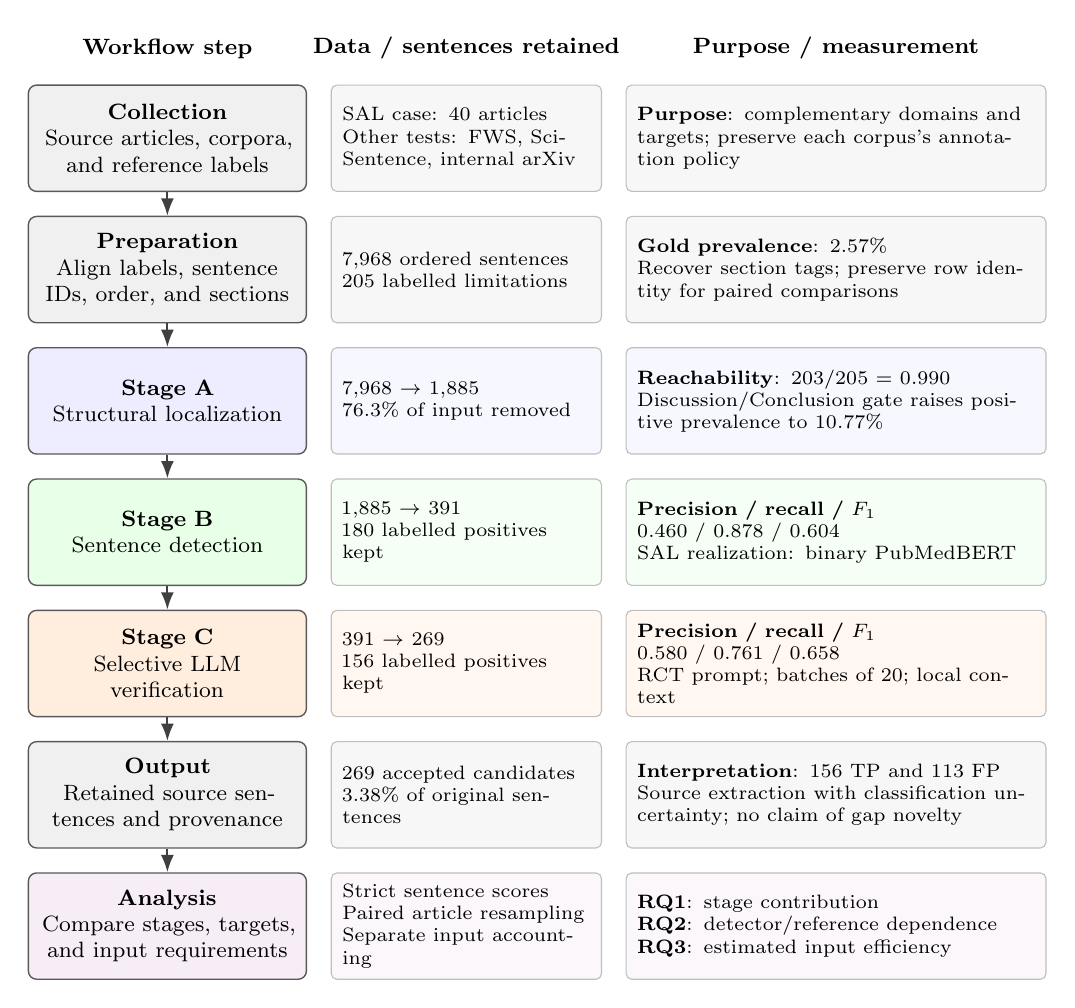
\begin{tikzpicture}[
 font=\footnotesize, node distance=3mm,
 stage/.style={draw=black!65, rounded corners=3pt, align=center, text width=3.25cm,
 minimum height=1.35cm, inner sep=4pt, line width=.5pt},
 cell/.style={draw=black!25, rounded corners=2pt, align=left, font=\scriptsize,
 minimum height=1.35cm, inner sep=4pt},
 kept/.style={cell,text width=3.15cm}, metric/.style={cell,text width=5.05cm},
 head/.style={font=\footnotesize\bfseries,align=center},
 flow/.style={-{Latex[length=2.2mm]},line width=.7pt,black!75}]
\node[stage,fill=black!6] (data) {\textbf{Collection}\\ Source articles, corpora, and reference labels};
\node[stage,fill=black!6,below=of data] (prep) {\textbf{Preparation}\\ Align labels, sentence IDs, order, and sections};
\node[stage,fill=blue!7,below=of prep] (a) {\textbf{Stage A}\\ Structural localization};
\node[stage,fill=green!9,below=of a] (b) {\textbf{Stage B}\\ Sentence detection};
\node[stage,fill=orange!13,below=of b] (c) {\textbf{Stage C}\\ Selective LLM verification};
\node[stage,fill=black!6,below=of c] (out) {\textbf{Output}\\ Retained source sentences and provenance};
\node[stage,fill=violet!7,below=of out] (analysis) {\textbf{Analysis}\\ Compare stages, targets, and input requirements};
\foreach \x/\y in {data/prep,prep/a,a/b,b/c,c/out,out/analysis} \draw[flow] (\x)--(\y);
\node[kept,fill=black!3,right=3mm of data] (kd) {SAL case: 40 articles\\Other tests: FWS, Sci-Sentence, internal arXiv};
\node[kept,fill=black!3,right=3mm of prep] (kp) {7{,}968 ordered sentences\\205 labelled limitations};
\node[kept,fill=blue!3,right=3mm of a] (ka) {7{,}968 $\rightarrow$ 1{,}885\\76.3\% of input removed};
\node[kept,fill=green!4,right=3mm of b] (kb) {1{,}885 $\rightarrow$ 391\\180 labelled positives kept};
\node[kept,fill=orange!6,right=3mm of c] (kc) {391 $\rightarrow$ 269\\156 labelled positives kept};
\node[kept,fill=black!3,right=3mm of out] (ko) {269 accepted candidates\\3.38\% of original sentences};
\node[kept,fill=violet!3,right=3mm of analysis] (kr) {Strict sentence scores\\Paired article resampling\\Separate input accounting};
\node[metric,fill=black!3,right=3mm of kd] (md) {\textbf{Purpose}: complementary domains and targets; preserve each corpus's annotation policy};
\node[metric,fill=black!3,right=3mm of kp] (mp) {\textbf{Gold prevalence}: 2.57\%\\Recover section tags; preserve row identity for paired comparisons};
\node[metric,fill=blue!3,right=3mm of ka] (ma) {\textbf{Reachability}: 203/205 = 0.990\\Discussion/Conclusion gate raises positive prevalence to 10.77\%};
\node[metric,fill=green!4,right=3mm of kb] (mb) {\textbf{Precision / recall / $F_1$}\\0.460 / 0.878 / 0.604\\SAL realization: binary PubMedBERT};
\node[metric,fill=orange!6,right=3mm of kc] (mc) {\textbf{Precision / recall / $F_1$}\\0.580 / 0.761 / 0.658\\RCT prompt; batches of 20; local context};
\node[metric,fill=black!3,right=3mm of ko] (mo) {\textbf{Interpretation}: 156 TP and 113 FP\\Source extraction with classification uncertainty; no claim of gap novelty};
\node[metric,fill=violet!3,right=3mm of kr] (mr) {\textbf{RQ1}: stage contribution\\\textbf{RQ2}: detector/reference dependence\\\textbf{RQ3}: estimated input efficiency};
\node[head,above=2mm of data] {Workflow step};
\node[head,above=2mm of kd] {Data / sentences retained};
\node[head,above=2mm of md] {Purpose / measurement};
\end{tikzpicture}

\caption{Workflow from collection and preparation to research-question analysis.
Counts illustrate the saved SAL realization: recovered
Discussion/Conclusion tags, a binary PubMedBERT detector, and RCT-prompt verification. Other
experiments use the configurations in \Cref{S:stage-a,S:stage-b,S:stage-c}; the hybrid runner
and raw-PDF parsing are not evaluated by these SAL counts.}
\label{F:pipeline}
\end{figure}

\subsection{Task definition}
\label{S:task}

The principal task returns sentences expressing a limitation of the authors' own study or a
future-work direction associated with that study. A limitation may concern study design, data,
evaluation, assumptions, or applicability. A future-work statement proposes subsequent research
rather than merely describing a contribution already made. The system does not determine whether
an author-stated problem is still open in the wider literature.

Let a parsed article be $D=(s_1,\ldots,s_n)$. Stages produce nested index sets
\begin{equation}
 I_C\subseteq I_B\subseteq I_A\subseteq\{1,\ldots,n\}.
\end{equation}
An output contains the retained source sentence, paper identifier, predicted type, section label,
acceptance source, confidence value, and local context. Text is selected rather than rewritten.
This guarantees extraction from the \emph{parsed representation}, not perfect correspondence to
PDF typography or correct attribution. Parsing and classification errors remain possible. Rule
confidence is a fixed value and classifier confidence is a model probability; neither is treated
as a calibrated measure of factual correctness.

The Sci-Sentence auxiliary experiment uses a different positive definition: Limitation or
Research Gap, including statements about prior work. Its target-matched verifier permits that
attribution. These results are reported separately from the principal task. Threats to validity
can trigger a target-section rule, but no independently evaluated third output class is claimed.

\subsection{Evaluation data and evidence provenance}
\label{S:data}

\Cref{T:datasets} lists the evaluated subsets rather than conflating them with the size of each
upstream resource. The principal SAL artifact contains 40 articles, 7,968 ordered sentences, and
205 limitation labels. Its records include article identifiers, recovered section tags, gold
labels, and predictions from eight detectors. Section tags were recovered through PMC BioC in the
original experiment. This reconstruction is held fixed in our offline analysis; its quality is not
established by the sentence-classification metrics.

\begin{table}[t]
\centering
\small
\caption{Evaluation subsets and the surviving evidence used in the present study.
``Aggregate'' means that complete row-level predictions were not supplied for independent recomputation.}
\label{T:datasets}
\begin{tabularx}{\linewidth}{@{}>{\raggedright\arraybackslash}p{2.6cm}>{\raggedright\arraybackslash}p{3.3cm}YY@{}}
\toprule
Subset & Size / target & Input condition & Evidence \\
\midrule
SAL/RCT \citep{lan2024automatic} & 40 articles; 7,968 sentences; 205 limitations & Reconstructed full-article stream; Discussion/Conclusion gate & Sentence labels, eight detector prediction vectors, and 391 verdicts for each of two prompts \\
SAL cost subset & 10 articles; 2,053 sentences; 55 limitations & Sample restricted to articles with at least two positives & Stage counts and full-article aggregate metrics; token estimates over all 40 articles \\
FWS \citep{zhang2023fws} & 1,506 sentences; 220 future-work positives & Curated future-work/conclusion material & Aggregate before/after filter metrics \\
Sci-Sentence \citep{bolanos2025scisentence} & 140 test sentences; 40 Limitation/Research-Gap positives & Curated rhetorical sentences; no localization gate & Aggregate baseline/filter metrics; additional target-matched runs recorded in notes \\
Internal arXiv reference & 10 articles; 49 mixed-type statements, including 11 limitations and 14 future-work statements & Parsed full articles; LLM-built silver labels & Notebook output and development summaries; original prediction files absent from the minimal snapshot \\
\bottomrule
\end{tabularx}
\end{table}

The SAL records are a reconstructed evaluation stream, not a new annotation effort. We do not
assume that an unlabelled sentence is certainly free of a semantically valid limitation, nor
replace source labels on the basis of an LLM's disagreement. The FWS breadth script removes exact
training-sentence matches and samples papers with seed~0 until the selected pool reaches about
1,500 sentences. This sentence exclusion is not proof of complete paper-disjointness.
Sci-Sentence uses its supplied 140-sentence test partition. Raw upstream files and trained checkpoints are not included in the minimal branch. A
new regenerator supplies the binary frozen-head recipe; exact checkpoint-level regeneration
remains distinct from recomputing metrics from the saved predictions.

The internal 49-statement set contains scope, assumption, and open-problem labels in addition to
the two detector classes. We use its target-specific limitation and future-work recalls only;
recall over all 49 labels would have a different denominator and a different task definition.
These labels were produced by an LLM and should be described as silver reference annotations.
They neither establish human annotation agreement nor support precise system precision, because
negative sentences were not exhaustively annotated. The original internal reference is separate
from the older unarXive section-overlap benchmark.

\subsection{Collection, preparation, and label alignment}
\label{S:preparation}

The workflow begins by selecting a source corpus and recording its document identifiers, native
annotation units, and intended target. This precedes model selection: a limitation-only biomedical
benchmark, a future-work sentence collection, and a rhetorical-role corpus cannot be made
interchangeable merely by giving their positive labels the same name. The public resources
supply complementary tests of the extraction components; the internal articles exercise parsing
and transfer under a smaller, less reliable reference. We retain these distinctions when choosing
eligible inputs and interpreting their outcomes.

For the SAL analysis, the collected material is the saved sentence stream and its recovered
PMC section metadata. Article identifiers and sentence order connect the gold labels, section gate,
detector predictions, and verifier verdicts. Preparation therefore preserves the row identities
through every stage rather than independently resegmenting text for each model. This permits
paired stage comparisons and prevents a removed sentence from disappearing from the recall
denominator. The exact upstream reconstruction and any excluded source records must be recovered
before rebuilding this stream from the original corpus; the present analysis starts from its
saved 7,968 records.

FWS provides already curated sentences. Its breadth evaluation loads the available test material,
excludes exact sentence matches to the training text, and selects the documented seeded subset.
Sci-Sentence supplies a fixed test partition and rhetorical labels; Limitation and Research Gap
are merged for its binary test. These preprocessing choices are explicit because curated
sentences test recognition and verification, whereas reconstructed article streams additionally
test localization. A train/test split should be tracked by article identifiers as well as text:
exact sentence deduplication alone cannot exclude near duplicates or other sentences from the
same article.

For raw articles, preparation instead extracts text blocks, identifies headings, segments
sentences, and associates each sentence with its source section. The PDF libraries provide a
local, inspectable route that can retain layout cues without requiring an external parsing service.
The resulting record must preserve enough source information to inspect errors in reading order,
segmentation, and heading assignment. This route is implemented in the runner, but the SAL
experiment's recovered tags do not demonstrate its accuracy. We distinguish an error caused by
an absent candidate region from a detector error on an available sentence.

Label alignment is likewise recorded before scoring. Our principal definition excludes criticism
of prior work unless the sentence also states a limitation or direction of the present study.
For example, an authors' statement that their sample covers only one institution fits the
limitation target; a claim that earlier methods ignore a phenomenon does not automatically fit it.
A proposal to test a method on additional populations fits future work, while a description of an
experiment already completed does not. These are illustrative policy examples, not additional
annotated observations. Sci-Sentence's broader binary target is retained under its own definition;
its Research Gap labels are not silently reannotated to match the author-only task.

\subsection{Stage A: structural localization}
\label{S:stage-a}

The reusable runner invokes \texttt{slice\_section\_aware}. It unions the mid-paper-anchor
localizer with complete sections whose headings name Discussion, Conclusion, Limitations,
Future Work, or related expressions. The anchor localizer combines spans after target headings,
inline keyword windows, the terminal tail, and narrow windows around scope/assumption phrases.
Generic discussion anchors are position-gated; explicit limitation and future-work anchors are
accepted independently of position. The terminal-window component caps selected units at 160; mid-paper additions and the
whole-section union can expand that set, so the final localizer has no global 160-sentence cap. The resulting region list removes
repeated source content according to the implementation's normalized-text keys.

For PDF input, \texttt{pdf\_to\_blocks} uses PyMuPDF, with pdfplumber as a fallback. Font size,
bold weight, and short-line/numbering cues distinguish headings from body text. The heuristic
uses a 1.12 body-font size ratio and a twelve-word heading limit. The sentence splitter protects
common abbreviations and applies text normalization; references and selected terminal headings
stop the eligible stream. These heuristics can introduce reading-order and sentence-boundary errors.

Structural localization is chosen as a low-cost, high-recall allocation mechanism. It reduces
how many sentences the detector and verifier inspect while retaining regions where authors often
qualify results or describe next steps. Whole-section retention protects statements without an
explicit cue, while anchor windows support less conventional article structures. The choice has
a direct measurable consequence: any labelled positive removed here is unreachable downstream.
We therefore assess both compression and positive reachability rather than treating a smaller
candidate pool alone as evidence of success.

The principal SAL experiment uses a simpler, explicitly distinct realization: retain sentences
whose recovered section tag is \texttt{DISCUSS} or \texttt{CONCL}. This measures localization
conditional on supplied section tags. It does not validate automatic heading recovery on PDFs.
In the FWS curated pool the gate is effectively a pass-through; in Sci-Sentence it is disabled.

\subsection{Stage B: sentence detection}
\label{S:stage-b}
\label{S:pipeline}

The reusable hybrid detector combines lexical cues with a frozen sentence encoder and a
class-weighted logistic regression. If a cue assigns a target label, that label is accepted;
otherwise the highest-probability classifier label must be a gap type and meet threshold
$\tau_B$. The cleaned runner uses \texttt{BAAI/bge-small-en-v1.5}, $C=2$, balanced class weights,
and $\tau_B=0.5$. Its expected training input is a cached self-distilled sentence set; development
notes describe ACL limitation augmentation. The cache itself is absent from this snapshot. If neither a head nor its training data is available, the runner falls back to
rules; that fallback must not be reported as a classifier run.

The final Stage-B notebook instead selects a frozen MiniLM-L6 encoder with logistic regression
trained on Sci-Sentence, FWS, and SAL. These are separate configurations. Its training label map
collapses Sci-Sentence Research Gap and Extension into the label named \emph{future work} and
Limitation into \emph{limitation}. This is a proxy mapping: an Extension sentence is not necessarily
future work. That semantic mismatch is a transfer limitation, not a change to the task definition.
The development comparison also includes bge-base, e5-base, mpnet, and full fine-tuning of
DistilBERT, SciBERT, and PubMedBERT~\citep{sanh2019distilbert,beltagy2019scibert,gu2021pubmedbert}.
Frozen sentence features are obtained through Sentence-Transformers~\citep{reimers2019sentencebert}.

Frozen encoders with a linear head separate semantic representation from task-specific fitting.
They provide a comparatively small adaptation component and allow several representations to be
compared without fine-tuning the entire encoder. Balanced class weights counter the dominance of
non-target training sentences, and logistic regression supplies probabilities for thresholding.
The regularization parameter and threshold specify the implemented operating point; they are not
claimed to be universally optimal. Lexical cues offer an explicit path for conventional limitation
and future-work expressions, but may confuse hypothetical statements, prior-work descriptions,
and generic conclusions. The semantic head complements this path by recognizing wording beyond
literal cue matches.

Fine-tuned scientific and biomedical encoders test a different adaptation strategy. Their inclusion
asks whether representations specialized for scientific text and its domain improve detection on
the evaluated stream. A detector ranking can reflect domain, training data, optimization, and
threshold choice simultaneously. Accordingly, the saved-vector comparison answers which recorded
configuration performed better; it does not isolate pretraining architecture as the sole cause.

In the SAL experiment, Stage~B consists of eight saved binary detector prediction vectors: five
frozen encoder heads and three fine-tuned encoders. Their names are retained in the result tables.
The analysis applies Stage~A to those predictions and compares them on the same source labels.
The supplied \texttt{dump\_sal\_preds.py} regenerates the five frozen columns using normalized
embeddings, balanced logistic regression ($C=2$, maximum 2,000 iterations), SAL's training CSV,
and a default positive-probability threshold of 0.5. It parses the list-valued
\texttt{limitation\_annotation} field and labels a sentence positive if any entry is true.
It preserves the three fine-tuned columns because their checkpoints are not supplied. The
notebook describes SAL-specific fitting and threshold tuning, but complete fine-tuning run
manifests remain unavailable. Thus a specified frozen-head regeneration recipe does not establish
bit-for-bit reproduction of every saved encoder or fine-tuned checkpoint.

\subsection{Stage C: selective verification}
\label{S:stage-c}

The API verifier receives candidate sentences and returns structured \texttt{\{id, keep\}}
judgments. It uses temperature zero, a strict JSON schema, and retries missing batch judgments
through the single-item path. Empty single-item responses are handled conservatively by keeping
the candidate; this is a failure policy, not a guarantee of semantic correctness. Surviving
sentences are not rewritten.

The saved SAL run uses \texttt{yandexgpt-5-lite}, batches of 20 candidate sentences in document
order, and at most one neighboring sentence on each side within the same article. It judges the
actual PubMedBERT-positive stream rather than the union of positives from several detectors.
Two cached prompt configurations are available: the keep-biased RCT prompt, labelled
\texttt{rct} in the verdict file, and a keep-biased SAL-criteria prompt, labelled \texttt{sal}.
Their complete target decisions are retained for all 391 candidates. The former depends on a
historical prompt alias not defined in the minimal branch; the latter's wording is present in
its experiment script. This provenance difference matters for regenerating API runs.

Verification is placed after detection because inspecting every full article with an LLM spends
input on a large number of obvious negatives. Local context supplies attribution and temporal cues
that an isolated candidate may omit: a preceding sentence can identify whose study is discussed,
and a following sentence can clarify whether an action is proposed or already completed. Keeping
context within the same article avoids attributing a candidate to an unrelated document. Batching
amortizes repeated instructions, but may affect attention and judgments; a batch of 20 is the
recorded configuration, not a demonstrated optimum.

The keep-biased instruction reflects the intended precision--recall trade-off. The verifier should
remove clear off-target candidates while avoiding unnecessary deletion of valid but indirectly
worded limitations. We therefore measure both false-positive removal and true-positive retention.
A better final precision accompanied by a large recall loss is not described as an unqualified
improvement. Structured identifiers connect decisions to their input rows and make the saved run
checkable; a well-formed JSON reply itself does not validate the content of those decisions.

The implementation also contains general author-gap and future-work prompt modes. In the
breadth experiment, FWS uses the future-work mode, whereas the initial Sci-Sentence run uses
the author-gap mode despite its different attribution target. Target-matched Sci-Sentence prompt
runs are treated as exploratory adaptation studies. The complete instruction is more than the selected base prompt. The shared batch wrapper
appends an authors'-own limitation/assumption/scope/future-work decision rule even when the
experiment overrides the base prompt. In particular, the intended gap-matched base prompt allows
prior-work gaps while that suffix rejects them. We retain these recorded runs as exploratory
configurations with conflicting instructions, rather than treating them as clean tests of target
alignment. The appendix records both layers; silently repairing the wrapper would produce a new
experiment, not reproduce the saved one.

The deployment runner protects selected cue
matches in explicit gap sections; the direct SAL verdict experiment judges every binary-detector
candidate. Batch size, context representation, judging order, and rule protection therefore
belong to the experiment configuration, not to an assumed universal default. The command-line
runner inherits a default batch chunk of 40 from \texttt{filter\_gaps}; the direct SAL experiments
explicitly use 20. The separate library entry point \texttt{extract\_all\_gaps} also restricts
model-only acceptance by section, unlike the runner's simpler cue-or-head rule. We do not assign
one implementation's measurements to every entry point.

\subsection{Experimental design and comparisons}
\label{sec:experimental-design}

The design links each research question to a unit of analysis, a comparison, and a measurable
answer (\Cref{T:rq-design}). The article is the sampling unit for uncertainty estimation, while
sentence-level labels determine extraction correctness. Dataset-specific findings are kept
separate so that differences in input preparation and annotation policy remain visible.

\begin{table}[t]
\centering\small
\caption{Operational design and justification for answering each research question.}
\label{T:rq-design}
\begin{tabularx}{\linewidth}{@{}p{1cm}YYY@{}}
\toprule
RQ & Comparison / analysis & Reported measures & Why these measures fit \\
\midrule
RQ1 & Same SAL rows: full detector, A+B, then A+B+C; both saved prompts & Reachability, candidate counts, precision, recall, $F_1$, TP retention, FP removal & Separates where candidates are lost from whether verification improves the surviving set \\
RQ2 & SAL detectors and classical baselines; auxiliary tasks; alternative references & Target-specific scores, candidate load, positional sensitivity, reference provenance & Separates detector behavior from label policy, reference coverage and test-pool differences \\
RQ3 & Forty-paper input accounting; separate ten-paper full-article pilot & Summed estimated input tokens and ratio; pilot extraction metrics and failures & Includes prompt/context overhead and checks effectiveness alongside input reduction \\
\bottomrule
\end{tabularx}
\end{table}

\paragraph{RQ1: stages on a common full-article stream.}
We recompute full-stream and A+B detector metrics from all 7,968 SAL records. We then apply the
cached RCT and SAL-criteria judgments to PubMedBERT's A+B candidates. The recall denominator remains
all 205 labelled limitations, including the two removed by Stage~A. This prevents conditioning
end-to-end recall only on reachable positives.

\paragraph{RQ2: detectors and annotation targets.}
The eight SAL detector vectors are compared under the same localization gate. Separate FWS and
Sci-Sentence tables use the saved aggregate metrics and explicitly state their input condition.
Development notes from the internal arXiv set report target-specific recalls and candidate load;
these are not full prediction-level replications. The aggregate baseline grid includes an all-negative predictor, cue rules, TF-IDF with
balanced logistic regression ($C=4$), binary one-to-four-gram counts with Bernoulli naive Bayes,
and normalized bge-small embeddings with balanced logistic regression ($C=2$). Feature extraction
is fitted on training material. SAL uses the saved full stream; FWS uses a separate seeded
20\%-of-paper test split; Sci-Sentence uses its supplied test partition. The FWS baseline grid
and 1,506-sentence breadth pool therefore have different test memberships and are not paired.
A second development notebook compares TF-IDF/SVM, training-only chi-squared feature selection
with Bernoulli naive Bayes, frozen heads, and SciBERT fine-tuning on its own grouped splits.
Those logged tables remain separate from the saved native-prevalence grid.

We do not pool the datasets or compare binary
positive-class $F_1$ directly with a seven-class or macro-averaged published score.

\paragraph{RQ3: input accounting and a small full-article comparison.}
The accounting file estimates full-article and selective-verification input on all 40 SAL papers.
It uses \texttt{cl100k\_base} tokens, includes repeated prompts and surrounding context, and assumes
per-paper batching at 20 candidates. Prompt/message wrappers contain approximate overhead constants.
It is not a reconstruction of exact billed requests for the separately cached verifier stream.
We report summed inputs and their ratio, excluding output tokens, embedding computation, model
training, and API retries.

The full-article baseline sends numbered article sentences to the same Yandex model and extracts
returned sentence indices. Its recorded run covers ten articles selected with seed~1 from papers
having at least two labelled limitations. It uses a separate extraction prompt and does not implement
chunking or a strong retry policy. Failed/unparseable replies yield no extracted indices. The
recorded two empty/unparseable cases are part of that baseline's outcome, not removed from its
reported recall denominator. The small sample is not representative of all papers, and the
comparison does not isolate localization from prompt and output-format differences.

\paragraph{Selection and uncertainty.}
Prompts, detector choices, and thresholds were inspected during development, including feedback
from benchmark subsets later used for reporting. The LLM comparisons are therefore exploratory.
For the complete SAL prediction/verdict pair, we additionally perform 10,000 paired
paper-cluster bootstrap resamples, with seed~20261013, recomputing pooled $F_1$ each time.
Percentile intervals describe variability conditional on the saved predictions. They do not
correct test-feedback selection, provider drift, or missing training provenance; no confirmatory
significance or non-inferiority claim is made. Aggregate-only studies receive no invented
confidence intervals or paired tests.

\subsection{Measures and reproducibility}
\label{S:measures}

Strict sentence scoring is primary. Positive-class recall measures whether the system finds the
annotated statements, while precision measures how much of the output a reader can accept under
the reference policy. Their harmonic mean summarizes the trade-off without concealing the
individual components. Accuracy would be dominated by the many negative sentences in the full
SAL stream and is therefore not the headline measure. Candidate counts additionally reveal the
work passed to subsequent stages, which a classification score alone does not capture.

Paper-cluster resampling preserves dependence among sentences from one article. Treating thousands
of sentences as independent samples would overlook their shared writing style, topic, and section
structure. Pairing the same resampled articles across stage configurations makes the difference
analyzed comparable within each resample. Where only pooled metrics survive, we report those
metrics at their recorded precision and avoid constructing article-level uncertainty from them.

With $TP$, $FP$, and $FN$ defined against the dataset's labels,
\begin{equation}
 P=\frac{TP}{TP+FP},\qquad R=\frac{TP}{TP+FN},\qquad
 F_1=\frac{2TP}{2TP+FP+FN}.
\end{equation}
We report positive-class metrics and the native prevalence of each evaluated subset when that
denominator is supplied. Development macro-$F_1$ values are labelled separately. Stage-A
reachability is the proportion of labelled positives retained; compression is the proportion of
all input sentences removed. Stage-C true-positive retention and false-positive removal are
computed relative to its input detector and the \emph{same gold labels}; they are not independent
of annotation error.

For the internal parsed-PDF reference, legacy matching uses normalized token containment at 0.7.
Token overlap tolerates boundary corruption but does not prove exact quotation or correct labeling.
We additionally recompute the repository's neighboring-sentence scores for windows $W=1,2$ as a sensitivity analysis: a prediction within $W$ positions of any gold sentence in the same paper contributes to
precision, and a gold sentence within $W$ positions of any prediction contributes to recall. This heuristic does not adjudicate
semantic equivalence and can credit multiple nearby predictions. It is not substituted for strict
scores or for manual review of disputed examples.

For prevalence sensitivity, we reuse the fixed SAL decisions inside the 1,885-sentence section
pool. All 203 reachable positives are retained and 778 negatives are sampled without replacement,
giving 981 sentences at approximately 20.7\% prevalence. We average $F_1$ over seeds 0--7 using
NumPy's default random generator. No new judging occurs after subsampling. This isolates the
scoring effect of negative sampling conditional on the saved decisions; it is not a reproduction
of the published authors' checkpoint or exact candidate pool.

\subsection{Reference construction and the human-validation protocol}
\label{S:reference-protocol}

The branch also documents an expanded model-labelled reference with three positive types:
limitation, future work, and research gap. The third label permits an unresolved issue in the
field or prior literature; it does not add a third independently evaluated output class to the
current two-target detector. The documented collection combines 190 arXiv CS/ML articles with
the same 40 SAL articles. Separate whole-paper model passes propose sentence indices and short
quotations. Quote checking is intended to verify source alignment. Agreement on the same type
forms one tier; an additional model pass adjudicates one-sided or type-disagreement candidates
to increase coverage. These tiers describe model agreement, not demonstrated human correctness.

Only the datasheet, the generated annotation interface, and its construction/merge utilities
are supplied. The raw full-corpus labels, model responses, collection manifest, and generation
scripts referenced by the datasheet are absent. Consequently, its corpus totals and inter-model
agreement are reported as documented construction statistics, separate from prediction-level
extraction results. Provider/model identifiers in that document have no accompanying request
logs or pinned versions; they are not evidence of a particular verified model release.

The implemented human-validation protocol samples four strata: 227 model-labelled limitation
sentences not labelled in SAL, 15 SAL-positive disagreement items, 60 positive controls, and
60 negative controls. The generated interface contains 362 numbered targets from 40 articles;
source/system labels are hidden, context is shown, and source articles are linked. Its builder
uses seed 13. Two annotators can record a binary decision, a type, and notes. The merge utility
computes coverage, raw agreement and Cohen's kappa on jointly answered rows; type agreement
is conditional on both annotators accepting the item as a gap.

The utility also reports consensus-only acceptance proportions and a lenient either-annotator
proportion. Disagreements are excluded from its consensus-only precision denominators; this is
not an independent adjudication procedure. The stratum-enriched sample cannot establish
population precision or full-corpus recall without appropriate sampling treatment and a
reference for items missed by all models. It covers the biomedical disagreement problem,
not independent validation of the 190 arXiv papers. No completed annotator exports or scored
human results are supplied, so this protocol contributes no human-agreement or corrected-precision
result in the present paper.

\subsection{Artifact-based reproduction}
\label{S:reproducibility}

The code snapshot examined is the \texttt{minimal} branch at commit \texttt{28a6c2d}. Our offline
verification records hashes of all 72 tracked files, verifies prediction/verdict coverage and
accounting totals, and generates the principal and supplementary numerical tables. No new detector training or LLM inference was performed
for that recomputation. Original experiments used GPU fine-tuning and API-based judging; CPU-capable
frozen heads are also implemented. Hard-coded machine paths, missing raw training inputs and
checkpoints, and API aliases ending in \texttt{latest} currently limit exact end-to-end reproduction.
The experiment prompts for SAL keep-biased and intended gap-matched validation are centralized
in \texttt{stage\_c\_prompts.py}; shipped prompts remain in \texttt{gap\_llm\_filter.py}.
The historical RCT alias is still imported from an absent helper. A changed detector stream
requires new matching verdicts: retaining an old cache after candidate changes is not a valid
pipeline rerun. The appendix distinguishes these regeneration constraints from the offline
score recomputation, which requires neither training nor paid inference.


\paragraph{Data and artifact availability.}
The analyzed code and saved outputs are identified by the
\href{https://github.com/Yazangthb/Gap2Idea/tree/28a6c2dbfad8ad332a66dd11e7b16f74d3ec4267}{repository commit}.
Public benchmark sources are attributed in \Cref{T:datasets}. The snapshot supplies the principal
SAL predictions/verdicts and several aggregate results, but not all training inputs, model
checkpoints, upstream reconstructions or expanded reference labels. Their absence limits
end-to-end regeneration; it does not prevent reproducing the principal saved-run scores.
Article text and benchmark data remain subject to their respective source licenses.

\section{Results}
\label{S:results}

The principal SAL tables are recomputed from saved row-level artifacts. The other tables distinguish
aggregate result files from development notes. All values describe the recorded configurations;
none is treated as an untouched-test estimate of a universal final pipeline.

\subsection{RQ1: localization, detection, and verification}

\paragraph{Localizer development.}
The internal ten-paper notebook retains executed outputs for the terminal-window and
mid-paper-anchor localizers. The former keeps 433 sentences and the latter 559, while reported
localization at 0.70 token containment rises from 0.633 to 0.857. Drop rates are 87.3\% and
83.6\%. This reference includes scope and assumption statements as well as limitations and
future work; these are region-coverage observations, not strict two-class extraction scores.
At 0.90 containment, localization is lower (0.429 and 0.633), showing dependence on the overlap
criterion. Full values and the logged section-aware comparison are in \Cref{A:development}.

The separate SAL-training development notebook reports five grouped-fold summaries of 0.861
mean reachability for anchor localization and 0.988 for whole target sections. The latter uses
supplied section names; it does not measure PDF heading recovery. Its cue-augmented count adds
potentially overlapping windows without full deduplication, so the archived augmented drop rates
are approximate. These summaries describe a development protocol with token-containment scoring;
they are not alternative estimates of the strict 40-paper evaluation below.

\paragraph{Fixed SAL test stream.}
Of 7,968 SAL sentences, 1,885 belong to the recovered Discussion or Conclusion sections.
This gate discards 76.3\% of the input while retaining 203 of 205 labelled limitations
(reachability 0.990). Prevalence rises from 2.57\% in the full stream to 10.77\% in the retained
pool. This is a conditional localization result using recovered tags rather than automatically
parsed PDF headings.

\begin{table}[t]
\centering
\small
\caption{SAL stage contributions on 40 articles, with all 205 labelled positives in the recall
denominator. TP denotes retained labelled positives. Both Stage-C rows use complete cached
judgments on the same 391 PubMedBERT candidates.}
\label{T:sal-stages}
% Auto-generated from exact saved prediction/verdict IDs
\begin{tabular}{@{}lrrrrr@{}}
\toprule
Configuration & Kept & TP & Precision & Recall & $F_1$ \\
\midrule
Stage A & 1885 & 203 & 0.108 & 0.990 & 0.194 \\
A+B: PubMedBERT & 391 & 180 & 0.460 & 0.878 & 0.604 \\
A+B+C: RCT prompt & 269 & 156 & 0.580 & 0.761 & 0.658 \\
A+B+C: SAL keep-biased & 249 & 148 & 0.594 & 0.722 & 0.652 \\
\bottomrule
\end{tabular}

\end{table}

\Cref{T:sal-stages} shows the resulting trade-off. PubMedBERT after localization retains
391 sentences, including 180 labelled positives. The RCT verifier removes 98 of the 211 detector
false positives (46.4\%), but also removes 24 of its 180 true positives. True-positive retention
is therefore 86.7\%. Precision increases from 0.460 to 0.580; recall decreases from 0.878 to 0.761;
$F_1$ increases from 0.604 to 0.658. The SAL keep-biased alternative retains fewer sentences
and achieves slightly higher precision, 0.594, but lower recall, 0.722, and $F_1$, 0.652.

The paired descriptive bootstrap interval for the RCT-prompt $F_1$ change is
$[0.026,0.083]$, around an observed increase of 0.054. The corresponding intervals for A+B and
A+B+C are $[0.554,0.654]$ and $[0.604,0.710]$. These intervals concern the saved-run comparison
only. Prompt refinement used benchmark feedback, so the positive interval does not establish a
confirmatory generalization claim.

An earlier notebook reports $F_1=0.701$ after judging a union of several detectors' candidates.
That run and the candidate-specific cached run are not interchangeable, because batch composition
and prompt configuration differ. We use the latter for the principal result. Nor is our full-stream
$F_1$ directly comparable to the published 0.821 recognition result of
\citet{lan2024automatic}, which used a different candidate-selection and model-development protocol.

\begin{table}[t]
\centering\small
\caption{SAL prevalence sensitivity with fixed predictions/verdicts. The section pool has
203 reachable positives; matching retains them and samples 778 negatives, averaging over eight
seeds. Full-stream scores retain all 205 positives in the recall denominator.}
\label{T:prevalence}
% Generated offline by revision_audit/verify_minimal.py
\begin{tabular}{@{}lrrrr@{}}
\toprule
Configuration & Full-stream $F_1$ & Pool recall & Pool $F_1$ & Matched $F_1$ \\
\midrule
A+B & 0.604 & 0.887 & 0.606 & 0.749 \\
A+B+C: RCT & 0.658 & 0.768 & 0.661 & 0.757 \\
A+B+C: SAL & 0.652 & 0.729 & 0.655 & 0.741 \\
\bottomrule
\end{tabular}

\end{table}

The recomputed prevalence analysis makes this distinction explicit (\Cref{T:prevalence}).
With negative subsampling to approximately 20.7\%, detector $F_1$ is 0.749, RCT-verified $F_1$
is 0.757, and SAL-verified $F_1$ is 0.741. Thus the RCT verifier's advantage narrows, and the SAL
variant no longer improves this measure. These are rescorings of fixed decisions, not new LLM
runs. They demonstrate dependence on the evaluated negative pool, without establishing a
universal prevalence threshold at which verification becomes useful.

Other prompt and model experiments have different judging populations. The stored
120-candidate balanced hard-sample sweep reports $F_1$ of 0.789, 0.779, and 0.784 for the three
Yandex variants. Aggregate union-candidate runs include the strict SAL result of 0.568 and
keep-biased SAL result of 0.554 for PubMedBERT; neither replaces its candidate-specific result
of 0.652. Model, prompt and batch membership differ across some runs, preventing attribution
of those differences solely to prompt wording. \Cref{A:verifiers} reports these development
results separately.

\subsection{RQ2: detector and reference dependence}

\begin{table}[t]
\centering
\small
\caption{Eight saved SAL detector vectors scored on the full stream and after the same
Discussion/Conclusion gate. These are positive-class metrics; the artifact permits metric
recomputation but does not fully reconstruct each training job.}
\label{T:sal-detectors}
% Auto-generated by revision_audit/verify_results.py
\begin{tabular}{@{}lrrrr@{}}
\toprule
Stage-B detector & Full-stream $F_1$ & A+B precision & A+B recall & A+B $F_1$ \\
\midrule
MiniLM-L6 (frozen) & 0.216 & 0.249 & 0.727 & 0.371 \\
mpnet (frozen) & 0.280 & 0.304 & 0.776 & 0.437 \\
bge-small (frozen) & 0.282 & 0.298 & 0.810 & 0.436 \\
bge-base (frozen) & 0.294 & 0.299 & 0.815 & 0.437 \\
e5-base (frozen) & 0.314 & 0.312 & 0.849 & 0.457 \\
DistilBERT-FT & 0.413 & 0.377 & 0.849 & 0.523 \\
SciBERT-FT & 0.458 & 0.405 & 0.873 & 0.553 \\
PubMedBERT-FT & 0.495 & 0.460 & 0.878 & 0.604 \\
\bottomrule
\end{tabular}

\end{table}

Localization raises $F_1$ for every saved SAL detector vector (\Cref{T:sal-detectors}).
PubMedBERT has the highest A+B $F_1$ in this comparison, followed by SciBERT and DistilBERT.
The frozen heads retain useful recall but produce more false positives. This supports the
localization mechanism for these fixed predictions; it does not establish that parameter count,
pretraining domain, or fine-tuning alone caused the observed ranking.

\paragraph{Classical and frozen baselines.}
The saved native-prevalence baseline grid is reported in \Cref{T:baseline-grid}. On the full
SAL stream, TF-IDF/logistic regression has $F_1=0.443$, compared with 0.273 for its separately
fitted bge-small head; the cached bge-small column in \Cref{T:sal-detectors} has 0.282. These are
different saved fits, not rounding variants of one run. On the grid's FWS split, TF-IDF/logistic
regression reaches 0.714, and on binary Sci-Sentence the in-domain bge-small head reaches 0.814.
All-negative predictions have zero positive-class $F_1$. These results establish useful
classical baselines and show why encoder size alone is an inadequate explanation of performance.
The FWS grid score must not be treated as a paired comparison with the 0.707 breadth result,
because their test pools differ.

\begin{table}[t]
\centering\small
\caption{Saved baseline-grid aggregates: positive-class metrics. SAL uses the 7,968-row full
stream; FWS uses a separate paper-level 20\% holdout, whose exact test count is not stored in
the aggregate; SciSentence uses the supplied 140-row binary test.}
\label{T:baseline-grid}
% Generated offline by revision_audit/verify_minimal.py
\begin{tabular}{@{}llrrr@{}}
\toprule
Subset & Method & Precision & Recall & $F_1$ \\
\midrule
SAL & majority (all-neg) & 0.000 & 0.000 & 0.000 \\
SAL & TF-IDF + LogReg & 0.362 & 0.571 & 0.443 \\
SAL & CountBin(1-4) + BernoulliNB & 0.000 & 0.000 & 0.000 \\
SAL & cue-rules only & 0.355 & 0.215 & 0.267 \\
SAL & bge-small frozen + logreg & 0.164 & 0.820 & 0.273 \\
FWS & majority (all-neg) & 0.000 & 0.000 & 0.000 \\
FWS & TF-IDF + LogReg & 0.667 & 0.767 & 0.714 \\
FWS & CountBin(1-4) + BernoulliNB & 0.880 & 0.510 & 0.646 \\
FWS & cue-rules only & 0.855 & 0.559 & 0.676 \\
FWS & bge-small frozen + logreg & 0.514 & 0.820 & 0.632 \\
SciSentence & majority (all-neg) & 0.000 & 0.000 & 0.000 \\
SciSentence & TF-IDF + LogReg & 0.784 & 0.725 & 0.753 \\
SciSentence & CountBin(1-4) + BernoulliNB & 0.895 & 0.425 & 0.576 \\
SciSentence & cue-rules only & 1.000 & 0.150 & 0.261 \\
SciSentence & bge-small frozen + logreg & 0.761 & 0.875 & 0.814 \\
\bottomrule
\end{tabular}

\end{table}

\begin{table}[t]
\centering
\small
\caption{Aggregate breadth results. FWS targets author-stated future work; Sci-Sentence merges
Limitation and Research Gap and includes prior-work criticism. Neither row evaluates raw-PDF
localization. The Sci-Sentence filter here uses the author-gap prompt and is deliberately
reported as a target mismatch.}
\label{T:breadth}
\begin{tabular}{@{}llrrr@{}}
\toprule
Subset & Configuration & Precision & Recall & $F_1$ \\
\midrule
FWS ($n=1{,}506$) & A+B & 0.723 & 0.618 & 0.667 \\
 & A+B+C, future-work prompt & 0.843 & 0.609 & 0.707 \\
Sci-Sentence ($n=140$) & Detector & 0.578 & 0.650 & 0.612 \\
 & Detector+C, author-gap prompt & 0.900 & 0.450 & 0.600 \\
\bottomrule
\end{tabular}
\end{table}

The aggregate FWS run raises precision with little recorded recall loss, whereas the
Sci-Sentence run raises precision at a larger recall cost and slightly reduces $F_1$
(\Cref{T:breadth}). The latter's label definition permits prior-work gaps that an author-gap
prompt rejects. Subsequent notes record target-matched prompt and in-domain threshold adaptation,
but complete decisions for those additional runs are not available in the supplied snapshot.
The development log reports $F_1=0.730$ for the intended gap-matched prompt with the existing
cross-domain detector, and 0.880 for an in-domain bge-small head at threshold 0.3 followed by
that prompt. Before verification, the latter retains 39 of 40 positives among 61 candidates;
after verification it retains 33 positives among 35 candidates. These logged counts are
arithmetically consistent with precision 0.943 and recall 0.825, but their full decisions are
not supplied. The contradictory shared prompt suffix described in \Cref{S:stage-c}, together
with test-informed development, limits interpretation as a clean policy-alignment experiment.
\Cref{A:breadth-adaptation} records the configurations; none is an independent confirmation
that the verifier is nearly error-free.

\begin{table}[t]
\centering
\small
\caption{Internal arXiv development notes, restricted to the 11 limitation and 14 future-work
reference statements. The 49-statement mixed-type denominator is not used. Retained-sentence
counts indicate candidate load, not validated precision. No new training replication was performed.}
\label{T:transfer}
\begin{tabular}{@{}lrrr@{}}
\toprule
Rules + detector & \shortstack{Limitation\\recall} & \shortstack{Future-work\\recall} & \shortstack{Retained\\sentences} \\
\midrule
bge-small (frozen; mixed-source training) & 0.545 & 0.786 & 97 \\
MiniLM-L6 (frozen; mixed-source training) & 0.636 & 0.857 & 170 \\
mpnet (frozen; mixed-source training) & 0.455 & 0.786 & 186 \\
PubMedBERT (fine-tuned; mixed-source training) & 0.364 & 0.714 & 65 \\
\bottomrule
\end{tabular}
\end{table}

The internal reference illustrates a different operating-point trade-off
(\Cref{T:transfer}). MiniLM retains more target statements and more candidates than bge-small.
The full fine-tuned model has lower recorded target recall on this small silver set. The result
cannot establish that frozen encoders generally transfer better: the set is small, its reference
coverage is incomplete, training-label mappings differ from the principal task, and precision
was not independently measured. It also explains why the selected development notebook and the
portable runner currently name different default heads. The complete logged head-only and
hybrid comparisons, class-balancing checks, and within-corpus benchmark tables are retained in
\Cref{A:development}. Validation macro-$F_1$ and positive-reference recovery answer different
questions. Lower recovery after transfer is compatible with distribution shift, label-policy
mismatch, incomplete silver references, or overfitting; these observations do not isolate one
cause or establish a universal frozen-versus-fine-tuned ranking.

Alternative references further change the interpretation. The development notes describe a
33-statement two-target model reference and a stricter 19-statement reference. MiniLM's reported
recovery changes from 0.455 to 0.632, while Stage-A reachability changes from 23/33 to 14/19.
The latter reference was collected with incomplete reading of three long papers. This is
sensitivity to annotation coverage and policy on the same articles, not a measured system
improvement. The larger documented 230-paper reference and its pending human protocol are
summarized in \Cref{A:reference}. They supply no completed human accuracy result.

Neighbor-position scoring on the saved SAL stream also changes the numbers. For A+B, $F_1$
rises from 0.604 under strict scoring to 0.743 at $W=1$; RCT-verified output rises from 0.658 to
0.821. The latter number is coincidentally equal, after rounding, to the published SAL detector
score under a different protocol. It is not evidence of matching that system. Neighbor scoring
can credit multiple predictions around one gold sentence and does not establish semantic
correctness or repaired annotations (\Cref{T:neighbor}).

\subsection{RQ3: input volume and full-article prompting}

\begin{table}[t]
\centering
\small
\caption{Estimated input volume over the 40 SAL articles. The accounting includes repeated
verification prompts and local context, using \texttt{cl100k\_base} and approximate wrapper
constants. It excludes output tokens, inference latency, local detector work, and retries.}
\label{T:tokens}
\begin{tabular}{@{}lrr@{}}
\toprule
Input accounting & Total input tokens & Mean per article \\
\midrule
Full-article prompting & 282,846 & 7,071.2 \\
Selective verification & 75,622 & 1,890.6 \\
\bottomrule
\end{tabular}
\end{table}

The accounting file gives a ratio of $282{,}846/75{,}622=3.740$,
a 73.3\% reduction in estimated LLM input (\Cref{T:tokens}). Only 391 of 7,968 source sentences
reach verification, about 9.8 candidates per article. The token ratio is smaller than the
sentence-count ratio because repeated prompts and neighboring context contribute substantial
overhead. It is not a measured monetary saving, throughput increase, or constant per-article cost.

\begin{table}[t]
\centering
\small
\caption{Recorded ten-article SAL comparison: 2,053 sentences and 55 positives, sampled from
articles having at least two labelled limitations. The complete stage-count file survives;
full-article extraction survives as aggregate precision/recall and mean API input only.
The baseline $F_1$ is approximately 0.427, computed from its rounded precision and recall.}
\label{T:full-paper}
\begin{tabular}{@{}lrrrr@{}}
\toprule
Configuration & Kept & Precision & Recall & $F_1$ \\
\midrule
Stage A & 498 & 0.110 & 1.000 & 0.199 \\
A+B: PubMedBERT & 109 & 0.468 & 0.927 & 0.622 \\
A+B+C: RCT verifier & 77 & 0.584 & 0.818 & 0.682 \\
Full-article LLM & --- & 0.559 & 0.345 & $\approx$0.427 \\
\bottomrule
\end{tabular}
\end{table}

In this selected sample, A+B+C has higher recorded recall and $F_1$ than the full-article
baseline using the same model family (\Cref{T:full-paper}). The baseline's mean reported API input
is 6,540 tokens per article, while the 40-article accounting table concerns a different sample
and an estimated rather than billed input measure. We do not combine those two measures into a
sample-specific cost ratio. The baseline also lacks a robust chunking/retry protocol; two replies
were recorded as empty or unparseable. Consequently, the comparison includes both semantic
extraction and response-format robustness and is not evidence that a well-engineered full-article
LLM baseline, or a stronger model, would have the same performance.

\section{Discussion}
\label{S:discussion}

\subsection{What the stage comparison establishes}

The principal finding is a measured allocation trade-off. On the fixed SAL prediction artifact,
structural localization removes many non-target sentences with little loss of labelled positives.
The detector then reduces candidate load, and selective verification improves precision while
sacrificing some of the detector's recall. The RCT-prompt $F_1$ increase of 0.054 is useful for
this configuration, but its 13.3\% loss of detector true positives is also material. Verification
is therefore an optional operating-point choice, not a universally beneficial final step.

The result depends on where a stage is evaluated. A full-article detector sees a low-prevalence
stream, whereas curated conclusion sentences or a balanced recognition sample present a different
false-positive burden. Changing the negative sample changes precision and $F_1$ even when positive
recall is unchanged. Published values must consequently be matched by label definition, candidate
pool, prevalence, and metric before being treated as head-to-head comparisons.

\subsection{How the findings answer the research questions}

For RQ1, the stage counts explain both the gain and its cost. Localization retains almost all
labelled positives, whereas most of the final recall loss occurs in detection and verification.
A practitioner prioritizing discovery can retain the detector's broader candidate set; a reader
prioritizing a shorter review list may prefer the verified output. Both outputs preserve the
original sentence and can be exposed with their decision provenance. The experiment supports
this operating-point distinction rather than a single mandatory setting for every application.

For RQ2, the recorded SAL comparison favors the fine-tuned biomedical detector among the eight
saved vectors, while the separate full-stream baseline grid also shows a strong lexical baseline.
The breadth results caution against assuming that its ranking or verifier policy transfers unchanged.
Future-work recognition, own-study limitation recognition, and broader research-gap recognition
require different judgments. A reusable system should therefore expose the target policy and
its corresponding evaluation. The conflicting suffix in the current gap-matched experiment
also shows that policy must be checked in the assembled request, not just in the base prompt.
The present evidence is strongest for the saved SAL configuration and weaker for aggregate-only
transfer studies and silver-label internal observations.

For RQ3, selective processing provides a clear reduction in estimated verifier input under the
specified accounting profile. This result explains why the staged design is attractive when
many articles must be inspected. It does not determine the best overall deployment architecture:
a small local detector adds its own preparation and maintenance costs, and a hosted model's
response reliability affects both effectiveness and retries. These quantities should be measured
when making a system-level efficiency claim. The branch's projected cross-paper batching, prompt
caching and long-paper savings are scenarios rather than measured deployment improvements;
we do not promote them to billed-cost or throughput results.

\subsection{Attribution policy and reference labels}

The Sci-Sentence development experiments illustrate the importance of matching the intended
prompt policy to the reference task, although the conflicting shared wrapper prevents a clean
causal test of that change. A verifier instructed to reject criticism of prior studies can correctly follow that
instruction while disagreeing with a dataset that labels those criticisms as Research Gap or
Limitation. This is a target mismatch, not evidence that either definition is intrinsically wrong.
Likewise, a statement about a study's methodological constraint and an adjacent consequence can
be scored differently under sentence- or span-oriented guidelines.

Inspection of disagreements can reveal annotation ambiguities, missed labels, model errors,
and sentence-boundary errors. It cannot by itself establish that most false positives are correct
or that an LLM achieves a much higher ``true'' precision than its measured precision. Such a claim
requires independent, preferably domain-expert, adjudication of a representative disagreement
sample. We therefore retain the original benchmark labels in all reported metrics. Neighbor-credit
scores, if used, should be interpreted as positional sensitivity rather than corrected gold.

Source grounding has similar limits. Returning an existing parsed sentence avoids inventing the
sentence's wording, but does not establish that it is a genuine author-stated gap, that its subject
is the authors' own work, or that the gap remains unresolved. Future downstream systems would need
separate attribution, resolution, and novelty checks before using these extractions to propose research.

\subsection{Efficiency and deployment}

Selecting candidate sentences substantially reduces estimated LLM input in the measured SAL
accounting profile. The 3.74-fold ratio incorporates some repeated-prompt and context overhead,
which makes it more informative than simply quoting the percentage of sentences removed.
However, a complete system cost also includes parsing, embeddings, detector training and inference,
response retries, and output tokens. API billing depends on the actual tokenizer and provider
pricing. Prompt caching and cross-paper batching could change that profile, but their projected
savings are not measured deployment results here.

The ten-article full-LLM comparison is encouraging but limited. It uses one economical model,
one selected sample, a different extraction prompt, and a baseline with response-format failures.
A stronger comparison would hold the annotation policy fixed, save all responses, use equivalent
retry/chunking budgets, and measure both stage-wise effectiveness and actual resource use.
The present result should guide that evaluation rather than substitute for it.

\subsection{Implications for evidence-based research support}

An extracted statement is useful as a traceable starting point for literature analysis. It can
help readers locate a paper's qualifications, collect proposed follow-up studies, and compare
how a topic is framed across articles. Keeping the source wording and identifier allows those
readers to inspect the surrounding argument rather than relying on an isolated model summary.
However, aggregation requires further decisions: two sentences can express the same issue,
a proposed study may already have been completed, and a frequently mentioned limitation may
reflect reporting convention rather than scientific priority.

Broader human evaluation and venue-corpus analysis can address some of these questions. Such
analyses must connect their article samples, annotation definitions, and run configurations to
the extraction protocol. Annotation agreement, venue-level statement frequencies, and the
usefulness of generated research ideas each require their own measurements. They cannot be
inferred from a sentence-detection score or a reduction in verifier input alone.

\subsection{Threats to validity}

\paragraph{Selection and sampling.}
The verifier prompts were refined after inspecting benchmark feedback. Descriptive bootstrap
intervals capture variation among the saved articles, not the optimism introduced by that
selection. The next evaluation should freeze prompts, head, threshold, context, and batching before
examining an independent article set. The cost subset is additionally conditioned on at least two
labelled limitations per article; its outcomes need not describe papers with few or no such statements.
The FWS breadth selection excludes exact training sentences but does not certify exclusion of
all related or same-paper training material.

\paragraph{Measurement and transfer.}
Recovered BioC tags simplify full-article localization relative to noisy PDFs. Curated FWS and
Sci-Sentence inputs do not test that front end at all. The internal arXiv references and the larger documented reference are model-labelled.
The 362-row interface has no completed human results and samples biomedical disagreements,
so it cannot establish reference accuracy across both domains. Inter-model kappa is not a
substitute for human agreement. The small arXiv reference is silver,
positive-only, and contains an expanded label ontology; it supports limited target-specific
recall observations, not population accuracy or human agreement. Proxy training-label mappings,
including Extension to future work, further limit interpretation of cross-domain rankings.

\paragraph{Reproducibility.}
Principal SAL decisions survive and their scores can be checked without an API, but the fine-tuned detectors
still lack checkpoints and full training provenance; the newly supplied frozen-head regenerator
resolves only part of that gap. Some experiment scripts retain machine-specific paths or imports
of helpers absent from the minimal branch. Experiment base prompts have been centralized, but the historic RCT alias still needs to be
archived with its exact resolved wording. Models referenced through a provider's \texttt{latest}
alias may change, and temperature zero does not establish repeatability across versions or batch
compositions. Aggregate-only breadth and full-article results cannot support additional paired
significance analyses or error adjudication without their original predictions and responses.

These limits bound the current conclusions: a particular saved full-article funnel improves
its recorded precision and $F_1$, and selective processing reduces estimated input volume.
Independent human-annotated results, broader venue findings, and evaluated research-idea quality
are outside the evidence reported in this study.

\section{Conclusion}
\label{S:conclusion}

We studied an extractive funnel that localizes candidate regions, detects author-stated gap
sentences, and optionally verifies candidates with an LLM. In the reconstructed 40-article SAL
stream, localization retains 203 of 205 labelled limitations while discarding 76.3\% of sentences.
For the saved PubMedBERT predictions, selective verification raises precision from 0.460 to 0.580
and $F_1$ from 0.604 to 0.658, at a recall decrease from 0.878 to 0.761. These results answer RQ1
for the recorded configuration rather than for an independently frozen test protocol.

For RQ2, classical baselines, detector-development studies and auxiliary tasks show that
candidate load, domain, annotation target and reference coverage affect the operating point.
Group-partition localization summaries, alternative silver references and positional sensitivity
scores support narrower conclusions than a single pooled accuracy figure. A literature-gap label policy must not be silently
replaced by an authors'-own limitation policy. For RQ3, accounting on the 40 articles gives a
3.74-fold reduction in estimated LLM input; the selected ten-article baseline study records higher
funnel recall and $F_1$, but does not establish a general advantage over all full-article LLM methods.

The branch additionally supplies a model-labelled reference-construction account and a blind
human-validation interface. Their existence does not establish completed human validation.
The shared prompt-wrapper conflict should be resolved and the revised request frozen before
new inference is evaluated. The next step is an independent evaluation with frozen configurations, complete training and
prediction provenance, adjudicated errors, and measured total processing cost. Reliable source
extraction may support later idea-generation systems, but their novelty and usefulness require
separate experiments.

\appendix
\section{Configurations and supplementary experiments}
\label{A:configuration}

The manuscript concerns the \texttt{minimal} branch at \texttt{28a6c2d}. Source-level experiment
coverage is provided in the accompanying \texttt{EXPERIMENT\_COVERAGE.md}. Supplementary tables
preserve completed development comparisons without elevating notebook prose or aggregate-only
runs to the evidential status of saved sentence decisions. All comparisons retain their own
task, denominator, sampling procedure, and scoring convention.

\subsection{Implementation configurations and reproduction}
\label{A:implementation}

\begin{table}[H]
\centering\small
\caption{Distinct configurations in the branch. A shared stage decomposition does not imply
identical detector training or API requests.}
\label{T:configurations}
\begin{tabularx}{\linewidth}{@{}>{\raggedright\arraybackslash}p{2.6cm}YYY@{}}
\toprule
Configuration & Localization & Detection & Verification \\
\midrule
Command-line runner & Anchors union whole target sections; local PDF blocks & bge-small, cached three-class head; cues or threshold 0.5 & General/RCT base; protected rules; default chunk 40 \\
Final Stage-B notebook & Cached internal candidate regions & MiniLM, mixed Sci-Sentence/FWS/SAL; cues or head argmax & Not part of that notebook's metric \\
SAL primary test & Recovered Discussion/Conclusion labels & Eight saved binary vectors; PubMedBERT supplies 391 candidates & Two cached prompts, chunk 20, same-paper neighboring context, every candidate judged \\
FWS breadth & Curated sentences; pass-through & Production-style bge hybrid & Future-work mode, chunk 20 \\
Sci-Sentence adaptation & No section gate & Cross-domain hybrid or in-domain binary bge head & Intended gap override with conflicting shared suffix \\
\bottomrule
\end{tabularx}
\end{table}

The offline verifier checks all 391 candidate IDs against both cached verdict maps, recomputes
strict scores, paired bootstrap intervals, negative-subsampling sensitivity and positional
scores, and sums the token-accounting CSV. Source hashes and the complete tracked-file manifest
identify the analyzed snapshot. No training or API calls are required for these computations.
The new frozen-head regenerator specifies the five binary encoder-head recipes but requires the
external SAL training CSV. Fine-tuned predictions remain cached until their original checkpoints
are supplied. Both frozen-head regeneration and new judging are separate from score reproduction.

The principal SAL prediction fixture and its two complete verdict maps support offline scoring.
Separate files store the baseline-grid, breadth, token-accounting and ten-article pilot results.
Model and prompt sweeps preserve additional aggregate comparisons. Internal transfer and
public-benchmark development values survive in notebook reference tables and the Stage-B
result summaries; their referenced prediction/checkpoint files are not supplied. The companion
experiment inventory maps each result to its exact repository path and manuscript location.

\subsection{Localization and detector development}
\label{A:development}

\begin{table}[H]
\centering\small
\caption{Executed internal localizer outputs: ten articles, 49 mixed-type silver statements.
Localization is token containment within the concatenated selected region text, not one-to-one
sentence matching.}
\label{T:localizer-development}
\begin{tabular}{@{}lrrrrr@{}}
\toprule
Variant & Kept & Drop (\%) & Loc@0.70 & Loc@0.80 & Loc@0.90 \\
\midrule
Terminal windows (v1) & 433 & 87.3 & 0.633 & 0.551 & 0.429 \\
Mid-paper anchors (v2) & 559 & 83.6 & 0.857 & 0.735 & 0.633 \\
\bottomrule
\end{tabular}
\end{table}

The notebook's narrative states that section-aware v3 matches v2 on the fragmented internal
blocks; no independently executed v3 metric row survives. The final-notebook PDF front end is
implemented and demonstrated, but no exhaustive PDF parsing/heading accuracy study is supplied.
GROBID section slicing is also implemented as an alternative; its presence is not an evaluated
GROBID-versus-local-parser comparison.

\begin{table}[H]
\centering\small
\caption{Notebook reference values for SAL-training localization development. Values are means
and standard deviations across five article-grouped partitions. Reachability uses token
containment at 0.70. Cue-augmented drop accounting can count overlapping windows more than once.}
\label{T:localizer-cv}
\begin{tabular}{@{}lrr@{}}
\toprule
Selection rule & Reachability & Reported drop (\%) \\
\midrule
Anchor localizer & $0.861\pm0.054$ & 82.2 \\
Anchors + curated cues & $0.880\pm0.047$ & 79.5 \\
Whole target sections & $0.988\pm0.020$ & 75.8 \\
Whole sections + cues (logged) & $0.990\pm0.020$ & 75.4 \\
\bottomrule
\end{tabular}
\end{table}

The same development notebook reports single-split anchor reachability of 0.861/0.766/0.935
for train/validation/test and 0.882/0.798/0.946 after curated cues. It attributes the remaining
misses mainly to cue-less Discussion statements. These observations motivate whole-section
retention; their fold variability is descriptive, not a significance test. The archived cue
list is fixed across the grouped-fold summaries rather than re-mined inside every fold.

\begin{table}[H]
\centering\footnotesize
\caption{Logged detector development on the internal reference. SF means Sci-Sentence+FWS;
SFS adds SAL. Validation is pooled macro-$F_1$; L/F are limitation/future-work recovery against
11/14 silver reference statements. Head and hybrid columns share the cached localizer input.
Retained counts do not measure precision.}
\label{T:internal-full}
\begin{tabular}{@{}llrrrrrr@{}}
\toprule
Detector & Train & Val macro & Head L & Head F & Hybrid L & Hybrid F & Kept \\
\midrule
bge-small & SF & 0.633 & 0.273 & 0.714 & 0.455 & 0.786 & 104 \\
DistilBERT-FT & SF & 0.745 & 0.000 & 0.643 & 0.182 & 0.714 & 63 \\
SciBERT-FT & SF & 0.846 & 0.000 & 0.643 & 0.273 & 0.714 & 61 \\
bge-small & SFS & 0.718 & 0.364 & 0.786 & 0.545 & 0.786 & 97 \\
PubMedBERT-FT & SFS & 0.890 & 0.182 & 0.714 & 0.364 & 0.714 & 65 \\
bge-base & SFS & 0.742 & 0.273 & 0.786 & 0.455 & 0.786 & 76 \\
e5-base & SFS & 0.753 & 0.273 & 0.786 & 0.455 & 0.786 & 71 \\
mpnet & SFS & 0.668 & 0.364 & 0.714 & 0.455 & 0.786 & 186 \\
MiniLM-L6 & SFS & 0.656 & 0.364 & 0.714 & 0.636 & 0.857 & 170 \\
\bottomrule
\end{tabular}
\end{table}

The original SF training report describes 6,700 rows, including only 101 limitations, and
full fine-tuning with AdamW, learning rate $2\times10^{-5}$, three epochs and class-weighted
loss. The later mixed-source report lists 7,706 training rows. These are development mixtures,
not the command-line runner's unavailable self-distilled training cache. The larger frozen
representations have 768-dimensional embeddings; bge-small and MiniLM use 384 dimensions.
Reported validation macro-$F_1$ increases under full fine-tuning do not imply improved transfer.
The retained notes disagree on some per-dataset macro conventions; we use the consistent pooled
values and target-specific internal recoveries rather than mixing incompatible columns.

The MiniLM balancing notebook reports mixed-ontology recovery of 0.571 with balanced class
weights, 0.265 without weights, 0.551 with explicit resampling, and 0.571 with additional
paraphrases. The denominator is all 49 statements, including non-target types, and the
per-class decisions do not survive. These numbers document a development choice; they are
not two-target accuracy estimates or evidence that weighting is universally optimal.

Cue optimization is also recorded separately. On a paper-disjoint FWS development test, the
reported precision/recall/$F_1$ changes from 0.843/0.448/0.585 to 0.819/0.538/0.650 with curated
intent cues. Limitation-cue $F_1$ on SAL changes only from 0.267 to 0.275. A more permissive
future-keyword variant was rejected after development feedback and is not used as a held-out
performance claim. Its selection history further motivates caution about generalization.

\begin{table}[H]
\centering\small
\caption{Logged within-corpus benchmark development, separate from the saved baseline grid.
FWS is a balanced paper-grouped split, SAL samples about four negatives per positive from
training articles before a new split, and Sci-Sentence collapses seven labels into three proxy
classes on a new grouped split. Macro and positive/type $F_1$ are distinct measures.}
\label{T:within-corpus}
\begin{tabular}{@{}llrr@{}}
\toprule
Task & Method & Macro-$F_1$ & Positive/type $F_1$ \\
\midrule
FWS binary & Cues & 0.676 & 0.585 \\
 & bge-small & 0.836 & 0.833 \\
 & MiniLM & 0.791 & 0.787 \\
 & TF-IDF/SVM & 0.835 & 0.833 \\
 & Counts/chi-squared/NB & 0.837 & 0.829 \\
 & SciBERT-FT & 0.876 & 0.880 \\
\midrule
SAL binary & Cues & 0.581 & 0.256 \\
 & bge-small & 0.813 & 0.710 \\
 & MiniLM & 0.729 & 0.584 \\
 & TF-IDF/SVM & 0.833 & 0.735 \\
 & Counts/chi-squared/NB & 0.834 & 0.729 \\
 & SciBERT-FT & 0.900 & 0.843 \\
\midrule
Sci-Sentence proxy & bge-small & 0.714 & L 0.744; F 0.643 \\
 & MiniLM & 0.622 & L 0.667; F 0.517 \\
 & TF-IDF/SVM & 0.652 & L 0.458; F 0.684 \\
 & Counts/chi-squared/NB & 0.358 & L 0.087; F 0.356 \\
 & SciBERT-FT & 0.856 & L 0.706; F 0.916 \\
\bottomrule
\end{tabular}
\end{table}

These notebook reference tables do not establish superiority to the original papers' results:
the split, negative sampling, class maps and sometimes the averaging convention differ.
Earlier logged FWS recognition values (including 0.879 for bge-small) concern another run;
they are not substituted for the 0.836 macro-$F_1$ table above. Claims that an original FWS
result is inflated by leakage cannot be independently established from this branch's missing
reproduction outputs. Regularized fine-tuning and SPECTER2 are described as unrun or failed,
so they have no performance row. The older ACL-cap/self-distillation sequence is described in
a package README but not supported by completed outputs in the current all-experiments notebook.

Alternative model-built references on the internal articles contain 33 target statements
(40,000-character full-text cap) or 19 target statements in nine articles (9 limitations,
10 future-work statements). On the former, MiniLM recovery is 0.455 overall, 0.500 for limitation
and 0.421 for future work, with 23/33 reachable. On the latter, MiniLM and bge-small hybrid
recovery is 0.632, with per-type values 0.444/0.800 and 14/19 reachable; head-only recovery is
0.579. Their retained loads are 167/102 for the hybrids and 157/91 for the heads. Incomplete
reading of three long papers and differing annotation policies preclude treating either
reference as exhaustive human gold.

\subsection{Verifier model, prompt and judging-population experiments}
\label{A:verifiers}

\begin{table}[H]
\centering\small
\caption{Saved balanced hard-sample sweep: 120 detector candidates, 60 positive and 60 negative,
SAL keep-biased prompt, batches of 20. These selected-candidate results are not full-stream
extraction scores. Calls are the recorded counts, not dollar cost or latency.}
\label{T:verifier-sweep}
% Generated offline by revision_audit/verify_minimal.py
\begin{tabular}{@{}lrrrr@{}}
\toprule
Judge & Precision & Recall & $F_1$ & Calls \\
\midrule
yandexgpt-5-lite & 0.683 & 0.933 & 0.789 & 6 \\
yandexgpt-5-pro & 0.697 & 0.883 & 0.779 & 6 \\
yandexgpt-5.1 & 0.645 & 1.000 & 0.784 & 6 \\
\bottomrule
\end{tabular}

\end{table}

An earlier notebook implements a five-model by three-batch probe on 30 positive and 30 negative
SAL sentences (batch sizes 10, 20 and 40), but supplies no executed numerical table. Its qualitative
selection of the lite model at batch 20 is therefore a documented development decision, not an
independently checked optimum. A later context/batch/prompt diagnosis logs a best hard-sample
$F_1$ near 0.827 without full decisions or a recoverable configuration table. The development
summary also reports that 56/60 gold positives were kept in one mixed batch setting versus
37/60 in a denser stream. These observations motivate candidate-specific judging, but the
missing batch-level records prevent a controlled causal estimate of the batch effect.

\begin{table}[H]
\centering\small
\caption{Saved aggregate union-candidate runs. Strict SAL uses a different recorded judge/run
from the lite keep-biased variants; columns are not a controlled prompt-only ablation. Each
verifier run judged the union of 1,036 detector candidates before scoring a detector's subset.}
\label{T:union-runs}
% Generated offline by revision_audit/verify_minimal.py
\begin{tabular}{@{}lrrrr@{}}
\toprule
Detector & A+B $F_1$ & Strict SAL & SAL keep-biased & RCT \\
\midrule
MiniLM-L6 (frozen) & 0.371 & 0.490 & 0.445 & 0.435 \\
mpnet (frozen) & 0.437 & 0.519 & 0.471 & 0.472 \\
bge-small (frozen) & 0.436 & 0.533 & 0.484 & 0.482 \\
bge-base (frozen) & 0.437 & 0.527 & 0.484 & 0.465 \\
e5-base (frozen) & 0.457 & 0.536 & 0.499 & 0.490 \\
DistilBERT-FT & 0.523 & 0.556 & 0.544 & 0.537 \\
SciBERT-FT & 0.553 & 0.562 & 0.545 & 0.547 \\
PubMedBERT-FT & 0.604 & 0.568 & 0.554 & 0.567 \\
\bottomrule
\end{tabular}

\end{table}

An earlier broad-prompt union table survives only as notebook reference values. Its eight
A+B+C $F_1$ values are 0.576 (MiniLM), 0.623 (mpnet), 0.616 (bge-small), 0.620 (bge-base),
0.648 (e5-base), 0.691 (DistilBERT), 0.686 (SciBERT), and 0.701 (PubMedBERT). The candidate-specific
RCT result of 0.658 supersedes the latter as the principal deployment-stream estimate; differences
also involve run configuration. A verdict is not detector-independent when the model receives
several candidates jointly. The saved aggregate union runs demonstrate that verification can
also lower $F_1$: PubMedBERT's 0.604 A+B becomes 0.554 or 0.567 in the two keep-biased union runs.

A single-reader analysis in the development summary categorizes 22 of the SAL keep-biased
run's 101 false positives, suggesting a mixture of missed labels, policy differences, and
model errors. This is useful for hypothesis formation, but the sampling rule and independent
adjudication are unavailable. We neither replace the benchmark labels nor report the summary's
projected corrected precision.

The Kilicoglu cross-check is likewise a notebook-only report: 1,505 test sentences, approximately
31.8\% positive, bge/logistic detection at P/R/$F_1$ 0.719/0.781/0.749 and subsequent verification
at 0.876/0.503/0.639. No row predictions or implemented reproduction of the original authors'
rule-based baseline are supplied. This recorded precision increase and recall loss does not
establish widespread gold-label errors or evaluate the full PDF front end.

\subsection{Breadth adaptation and scoring sensitivity}
\label{A:breadth-adaptation}

\begin{table}[H]
\centering\small
\caption{Logged Sci-Sentence adaptation, all on the 140-sentence binary test. The base prompt
is intended to allow prior-work gaps but retains an incompatible authors'-own wrapper suffix.
Threshold/prompt selection was exploratory; complete row decisions are absent.}
\label{T:adaptation}
\begin{tabular}{@{}lrrr@{}}
\toprule
Configuration & Precision & Recall & $F_1$ \\
\midrule
Cross-domain hybrid + intended gap override & 1.000 & 0.575 & 0.730 \\
In-domain binary bge, threshold 0.5 & 0.761 & 0.875 & 0.814 \\
In-domain binary bge, threshold 0.3 & 0.639 & 0.975 & 0.772 \\
Same threshold 0.3 + intended gap override & 0.943 & 0.825 & 0.880 \\
\bottomrule
\end{tabular}
\end{table}

The in-domain Sci-Sentence script explores thresholds 0.5, 0.4, 0.3 and 0.2 and can judge the
last two settings. Only the reported settings above have supplied numerical summaries.
The analogous FWS recall-first script is implemented, with a different article split and
threshold sweep, but no completed output is supplied. Neither script's mere presence supplies
additional measured operating points. FWS disagreement examples are hypotheses about label
coverage, not adjudicated evidence of reference error.

\begin{table}[H]
\centering\small
\caption{Recomputed positional sensitivity on the fixed SAL decisions. Neighbor credit uses
many-to-many positional matching within each article; it is not a semantic span annotation or
an adjudicated correction of the benchmark.}
\label{T:neighbor}
% Generated offline by revision_audit/verify_minimal.py
\begin{tabular}{@{}lrrr@{}}
\toprule
Configuration & Strict $F_1$ & Neighbor $W=1$ & Neighbor $W=2$ \\
\midrule
A+B & 0.604 & 0.743 & 0.783 \\
A+B+C: RCT & 0.658 & 0.821 & 0.853 \\
A+B+C: SAL & 0.652 & 0.817 & 0.852 \\
\bottomrule
\end{tabular}

\end{table}

\subsection{Documented reference construction and pending validation}
\label{A:reference}

\begin{table}[H]
\centering\small
\caption{Construction totals reported in the branch's annotation datasheet. These values are
arithmetically consistent but not recomputed from the unavailable corpus/vote files. They are
model-labelled reference statistics, not independently validated extraction results.}
\label{T:reference-construction}
\begin{tabularx}{\linewidth}{@{}p{4.3cm}Y@{}}
\toprule
Item & Documented value \\
\midrule
Articles / sentences & 230 / 68,719 (190 arXiv articles and the same 40 SAL articles) \\
Positive statements & 4,462: 2,234 research gaps, 1,543 limitations, 685 future-work statements \\
Positive statements by domain & 3,751 arXiv; 711 SAL \\
Model-agreement / adjudicated tiers & 2,960 / 1,502 \\
Adjudication candidates & 1,737; 1,502 accepted and 235 rejected \\
Inter-model Cohen's kappa & Any gap 0.778; limitation 0.748; future work 0.869; research gap 0.725 \\
SAL reference recovery & Any-gap recall 0.956; limitation-specific recall 0.927 (190/205) \\
SAL limitation extras & 227; a further model pass accepts 116/227 (51.1\%) \\
Reported annotation expenditure & Approximately USD 37.5, including labeling, adjudication and the additional model pass \\
Human study & 362-row interface present; completed answers/results absent \\
\bottomrule
\end{tabularx}
\end{table}

The reported model strings are \texttt{claude-opus-5-5}, \texttt{claude-sonnet-5-5}, and
\texttt{claude-fable-5-1} with an Opus fallback. They are transcribed provenance identifiers
from the datasheet, not independently verified provider versions. No request/usage records
support exact rerunning or billing reconstruction. The 227 extras belong to this reference
construction, not to the 113 or 101 false positives of the two saved funnel configurations.
Likewise, limitation-specific recovery and any-gap recovery have different positive definitions.

Inter-model agreement must not be equated with human agreement or a human performance ceiling.
Another LLM's acceptance of 116 extras cannot determine that the remaining items are errors,
nor that the accepted ones are definitively correct. Quote alignment verifies text identity,
not label semantics. The planned human protocol in \Cref{S:reference-protocol} is an appropriate
next check, but supplies no completed validation result here. Its biomedical, disagreement-enriched
sample would not by itself validate every type and domain in the documented corpus.

\subsection{Exact surviving instructions and composition}
\label{A:prompts}

The verifier's batch schema returns a \texttt{results} array of integer \texttt{id} and Boolean
\texttt{keep}. Missing batch decisions fall back to a single-target call, which loses the supplied
neighbor context; an empty single-target response is kept conservatively. The current module
centralizes two experiment base prompts. The complete request additionally contains a shared
wrapper, calibration examples and numbered candidates. The following instruction is the surviving
SAL keep-biased base, followed by its examples.

% Extracted directly from SYS_SAL and SHOTS_SAL, not paraphrased.
\paragraph{SAL keep-biased system instruction.}
\begin{quote}\small
You judge whether the «marked» TARGET sentence is a SELF-ACKNOWLEDGED LIMITATION of the AUTHORS' OWN study, using the SAL annotation criteria. A limitation is a weakness/caveat/bias/constraint the authors admit about THIS trial, fitting a known category: study design; loose or narrow population / convenience sampling; single-center or narrow setting; intervention composite/non-standardized; control (no placebo / active placebo / care-as-usual); outcome measure excluded/imprecise/unvalidated; missing data or drop-out; small sample / underpowered; randomization unbalanced/poor/open; blinding (patient or team not blinded); short duration or follow-up; multiple/post-hoc testing or unadjusted confounding; funding; limited generalizability.

DECISION RULE (keep-biased):

- keep=true if the TARGET states such a limitation, OR states a consequence ('could introduce bias', 'cannot be assessed', 'results may be confounded', 'risk of type 1 error') whose underlying CAUSE (no blinding, small sample, single center, multiple testing, short follow-up...) is evident in the TARGET or its SURROUNDING context. When in doubt and a real weakness of this study is present, keep=true.

- keep=false ONLY for CLEAR non-limitations: restated positive results; clinical recommendations; critique of prior/other work; plain methods description; background; or a bare header like 'This study has several limitations.' with no specific weakness.

\end{quote}
\paragraph{Few-shot pairs.}
\begin{quote}\small
\noindent\textbf{YES}: the lack of a no treatment arm in this study\par
\noindent\textbf{YES}: our study included only a relatively small sample of participants\par
\noindent\textbf{YES}: The absence of masking is most relevant for the assessment of events.\par
\noindent\textbf{YES}: the crossover design and the relatively short treatment periods are limitations\par
\noindent\textbf{YES}: the trial was conducted at a single center\par
\noindent\textbf{YES}: Because outcomes were exploratory, the risk of type 1 error was considerable.\par
\noindent\textbf{YES}: This could have introduced a bias in the results.\par
\noindent\textbf{NO}: This study has several limitations.\par
\noindent\textbf{NO}: The intervention significantly reduced symptoms at 12 weeks.\par
\noindent\textbf{NO}: Clinicians should consider these findings when counseling patients.\par
\noindent\textbf{NO}: Existing methods cannot capture long-range dependencies.\par
\noindent\textbf{NO}: Participants were randomized 1:1 using a computer-generated sequence.\par
\end{quote}


\paragraph{Intended gap-matched base instruction.}
\begin{quote}\small
You are a precision filter for RESEARCH-GAP and LIMITATION statements in academic text, including related-work sections. KEEP the «marked» sentence if it identifies a limitation, weakness, shortcoming, unsolved problem, open challenge, or missing capability — in prior/existing work, a method, or the field (it need NOT be the authors' own study). DROP it if it merely describes what a work does, gives background, states results/findings, or makes a neutral or positive general statement with no gap or weakness. When a sentence clearly names a shortcoming or an unaddressed problem, KEEP.
\end{quote}
\noindent\textbf{Calibration pairs.}
\noindent\textbf{YES}: Existing methods cannot capture long-range dependencies.\par
\noindent\textbf{YES}: However, these approaches do not scale to large graphs.\par
\noindent\textbf{YES}: No prior work has addressed the multilingual setting.\par
\noindent\textbf{YES}: This remains an open problem in the field.\par
\noindent\textbf{YES}: Current benchmarks lack annotations for rare classes.\par
\noindent\textbf{NO}: archjava is an architecture description language on top of java.\par
\noindent\textbf{NO}: The model achieves 92\% accuracy on the benchmark.\par
\noindent\textbf{NO}: Smith et al. proposed a transformer-based model for this task.\par
\noindent\textbf{NO}: These tools are widely used in industry.\par


\paragraph{Shared decision suffix (verbatim).}
\begin{quote}\small
You will receive a NUMBERED list. For EACH item, decide keep=true if the TARGET states the AUTHORS' OWN limitation, assumption, scope restriction, or future-work direction, and keep=false otherwise (including limitations of prior or other work).

\end{quote}
This suffix conflicts with the gap-matched base's permission for prior-work criticism. Recording
it is necessary to interpret the saved results faithfully. The historical RCT-loose alias is
still imported from an absent helper and should not be replaced silently by the shipped RCT
instruction. Centralizing the SAL/GAP bases improves future maintainability but does not recover
that missing historical request.

\subsection{Evidence outside the reported experiments}
\label{A:excluded}

Historical LimGen binary-detection, BAGELS coverage and alternative FWS/SAL leaderboard values
appear in comparison notes without their producing scripts, checkpoints or predictions in this
snapshot. They establish development history, not independently checkable benchmark superiority.
The corresponding inventory entries record their values and exclusion reasons. Proposed
cross-provider LLM baselines, regularized fine-tuning and idea-generation evaluation have no
completed supporting results in this branch. Project plans are not experiment outcomes.

The previously discussed 64-article human study and 800-article venue corpus have no supplied
results in this snapshot. They are not replaced by the newer 362-row validation interface or
the documented 230-paper model-labelled collection: these are distinct samples and protocols.
No human agreement, venue distribution, temporal trend, or idea-generation quality is inferred
from their descriptions.


% ---------- Bibliography ----------
% plainnat/apalike/unsrtnat work with natbib's \citep / \citet
\bibliographystyle{plainnat}
% \bibliography{references}
\bibliography{references_handnotes}

% ---------- Appendix: Template usage examples ----------
% Remove this appendix once you no longer need the reference examples below.
% \appendix
% \section{Examples}
% \label{APX:examples}

% This appendix demonstrates the conventions used throughout this template. Copy whichever snippet you need into your own section files, then delete this appendix from your final report.

% \subsection{Figures}
% Place image files in \texttt{tikz/} and reference them as follows:

% \begin{figure}[H]
%     \centering
%     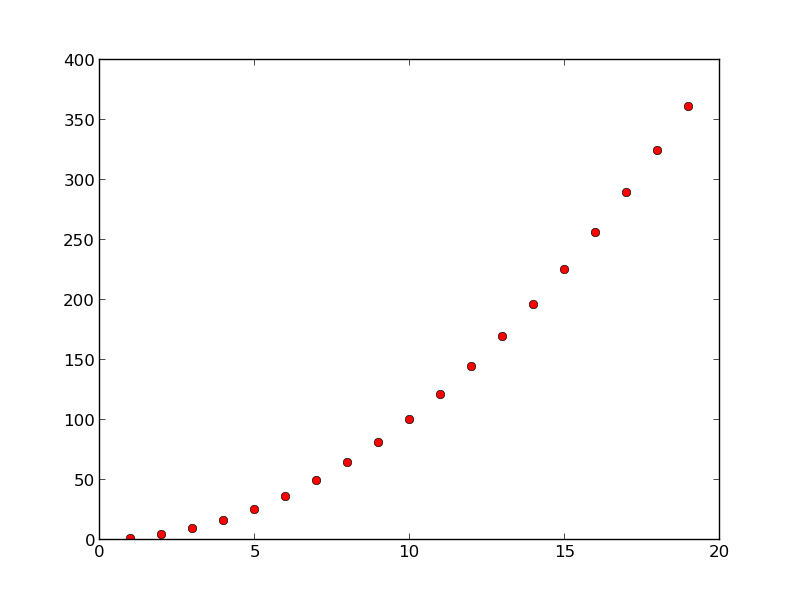
\includegraphics[width=0.6\textwidth]{tikz/example_plot.png}
%     \caption{Example figure. Replace \texttt{tikz/example-plot.png} with
%     your own file. Refer to it in text with \texttt{\textbackslash Cref\{F:example\}}.}
%     \label{F:example}
% \end{figure}

% As \Cref{F:example} shows, cleveref automatically inserts the word "Figure" for you — no need to type it manually.

% \subsection{Tables}
% For simple tables, use \texttt{booktabs} for clean horizontal rules (avoid vertical rules):

% \begin{table}[H]
%     \centering
%     \caption{Example results table.}
%     \label{T:example}
%     \begin{tabular}{lcc}
%         \toprule
%         Model & Accuracy (\%) & F1-score \\
%         \midrule
%         Baseline     & 72.3 & 0.68 \\
%         Proposed     & \textbf{81.5} & \textbf{0.77} \\
%         \bottomrule
%     \end{tabular}
% \end{table}

% \Cref{T:example} summarizes the comparison between the baseline and the proposed approach. For larger tables, save the \texttt{tabular} environment in its own file under \texttt{tables/} and pull it in with \texttt{\textbackslash input\{tables/your-table\}}.

% \subsection{TikZ figures}
% Students are encouraged to draw diagrams (flowcharts, experimental designs, architecture diagrams, decision trees, etc.) natively in \LaTeX{} using \texttt{TikZ} rather than pasting in screenshots — this keeps vector-quality, theme-consistent figures that scale cleanly in the PDF.

% \begin{figure}[H]
%     \centering
%     \begin{tikzpicture}[
%         node distance=1.5cm,
%         every node/.style={draw, rounded corners, align=center, minimum height=0.9cm},
%         arrow/.style={-{Latex[length=2mm]}}
%     ]
%         \node (start) {Collect Data};
%         \node (process) [right=of start] {Preprocess};
%         \node (analyze) [right=of process] {Run Experiment};
%         \node (result)  [right=of analyze] {Analyze Results};

%         \draw[arrow] (start) -- (process);
%         \draw[arrow] (process) -- (analyze);
%         \draw[arrow] (analyze) -- (result);
%     \end{tikzpicture}
%     \caption{Example TikZ diagram of an experimental pipeline.}
%     \label{F:tikz-example}
% \end{figure}

% For more complex diagrams, consider keeping the \texttt{tikzpicture} in its own file under \texttt{tikz/} and \texttt{\textbackslash input\{\}}-ing it, so \texttt{main.tex} stays readable.

% \subsection{Citations}
% This template uses \texttt{natbib}. Given a BibTeX entry with key \texttt{smith2020}, in \texttt{references.bib}:

% \begin{itemize}
%     \item \texttt{\textbackslash citep\{smith2020\}} renders as a parenthetical citation, e.g. \citep{smith2020} — use this when the citation is not the grammatical subject of the sentence.
%     \item \texttt{\textbackslash citet\{smith2020\}} renders as an in-text citation, e.g. \citet{smith2020} found that... — use this when you are directly discussing the authors' work.
% \end{itemize}

% \noindent\textit{Note:} \texttt{smith2020} is a placeholder key. Add real entries to \texttt{references.bib} before compiling, or these citations will show up as "\texttt{?}".

\end{document}
